\documentclass[11pt,a4paper]{article}

\usepackage[T1]{fontenc}
\usepackage{lmodern}
\usepackage[utf8]{inputenc}
\usepackage[margin=2.5cm]{geometry}
\usepackage{microtype}
\usepackage{amsmath}
\usepackage{amssymb}
\usepackage{amsthm}
\usepackage{booktabs}
\usepackage{array}
\usepackage{multirow}
\usepackage{graphicx}
\usepackage{xcolor}
\usepackage{float}
\usepackage[font=small,labelfont=bf]{caption}
\usepackage[round,authoryear]{natbib}
\usepackage[colorlinks=true,linkcolor=blue!50!black,citecolor=blue!50!black,urlcolor=blue!50!black]{hyperref}

% Typesetting helpers defined for this paper.
\newsavebox{\tabbox}
% Scale a table body down to the line width only when it is wider than the line.
\newcommand{\fittable}[1]{\sbox{\tabbox}{#1}%
  \ifdim\wd\tabbox>\linewidth\resizebox{\linewidth}{!}{\usebox{\tabbox}}\else\usebox{\tabbox}\fi}
\newcommand{\ci}[2]{$[#1,\,#2]$}
\newcommand{\pp}{\,pp}
\newcommand{\CE}{\mathrm{CE}}
\newcommand{\Cov}{\mathrm{cov}}
\newcommand{\MDE}{\mathrm{MDE}}
\newcommand{\Ind}{\mathbf{1}}

% Status of the language-model explainer evaluation: the single place to replace
% when results become available (used once in each section that mentions it).
\newcommand{\ExplainerStatus}{The evaluation of the language-model explanation layer is in progress and is not reported in this version; no claim of this paper depends on it.}

\title{Comparing Methods for Building Reliable Prediction Intervals for Machine-Learning Inflation Forecasts in Commodity-Dependent Economies}
\author{Nuraidyn Seitkapar}
\date{Draft of 19 November 2026}

\begin{document}
\maketitle

\begin{abstract}
\noindent
Prediction intervals for inflation inform decisions in commodity-dependent economies, but it is not known whether adaptive conformal methods that perform well on euro-area and US data keep their nominal coverage there. We build a multi-horizon (1, 3, 6 and 12 months) calibration benchmark of split, rolling-window, adaptive (ACI, FACI), conformal PID and regime-aware (DRACP) intervals at nominal level 0.90, using monthly IMF consumer price indices for 13 design economies, a first hold-out panel of 7 economies and, in an extension, a second hold-out panel of 10 economies, with LightGBM, ARIMA, a naive forecaster and the zero-shot foundation model Chronos as base forecasters. The primary outcome is the calibration error (CE), the mean over countries of $|\text{coverage}-0.90|$. Contrasts are tested with a moving-block bootstrap and Holm correction, equivalence of DRACP and ACI with two one-sided tests and a margin of 2 percentage points (pp), and decision rules R1--R5 were pre-specified in a version-controlled protocol before the hold-out run (a self-attested commit history; the rules were written after the exploratory results were known).

Adaptive methods had a lower calibration error than a calibration performed once and, in a post hoc comparison restricted to ARIMA, than the native intervals of that model; the direction is consistent across samples. The pre-specified rule R1 (ACI against split) was met only at a 96-month warm-up, a sensitivity run that is not promoted, and not at the primary 48-month warm-up (ACI minus split at $h=3$: $-3.0$~pp, $p=0.054$; at $h=6$: $-2.8$~pp, $p=0.092$). Whether ACI improves on a rolling window depends on the panel: it was not shown on the design panel and the first hold-out panel (minimum detectable difference undefined, inconclusive), and it was met under the pre-specified rule in part of the cells of the second hold-out panel at warm-up 48; the reason is not known and the panels are not pooled. DRACP against ACI is inconclusive, and because the 2~pp margin is about the size of ACI's own calibration error this verdict is weak by construction. No efficiency advantage in interval width or interval score is established. At the 12-month horizon pooled coverage is below nominal for every method on the design and first hold-out panels; in a diagnostic run that releases outcomes immediately, ACI coverage on the first hold-out panel was 2.4~pp higher (95\% interval $-0.1$ to $4.8$, which includes zero), below the pre-specified 3~pp threshold. On the 22 target months from 2025-01, a period that Chronos cannot be assumed to have seen in pretraining (its model card states no cutoff), its mean absolute error was lower than that of the naive baseline and, descriptively, at least as low as that of LightGBM and ARIMA. \ExplainerStatus{}
\end{abstract}


\section{Introduction}\label{sec:intro}

Central banks, finance ministries and firms in commodity-dependent economies use inflation forecasts, and a forecast is useful for decisions only together with a statement of its uncertainty. A prediction interval with a nominal level of 90 percent claims that in about nine cases out of ten the realised value falls inside it. Whether this holds is the question of calibration, and it can be checked against realised data; it is not guaranteed by the forecasting model, because the model's error distribution is estimated from a past that may not resemble the future.

Commodity-dependent economies are a demanding setting for calibration: their price levels are exposed to exchange-rate and commodity-price movements (\citealp{gelos2017commodity}), and their inflation regimes can change within a few years, for which we cite no source; it is the motivation for the setting and not a result, and the paper does not compare commodity-dependent economies with other economies (Section~\ref{sec:scope}). A calibration made once on a past window may fail later, and a method that adapts the interval width online is a natural candidate. Conformal prediction \citep{vovk2005algorithmic} gives distribution-free finite-sample coverage under exchangeability, which time series violate. Adaptive conformal methods \citep{gibbs2021aci,gibbs2024faci,angelopoulos2023pid,bhatnagar2023saocp} were designed for that case, and a recent regime-aware variant, DRACP \citep{oancea2026dracp}, reports mean coverage closest to nominal over 48 series including euro-area inflation. Conformal intervals have been applied to inflation in Brazil, Russia, India and China \citep{sengupta2025fewnet} and in Tunisia \citep{brahem2026tunisia}, but in the parts we read we found no comparison of the empirical coverage of several adaptive conformal methods. Whether DRACP-type results transfer to commodity-dependent economies and to multi-month horizons has therefore not been tested to our knowledge; this rests on a limited search (Section~\ref{sec:related}), not a systematic review.

\paragraph{Problem, gap and what is done.} The problem is the calibration of prediction intervals for the cumulative log growth of the consumer price index at horizons of 1, 3, 6 and 12 months in economies exposed to commodity and exchange-rate shocks. The gap is an evidence gap, not a methodological one. The closest work, \citet{oancea2026dracp}, evaluates DRACP on 48 macroeconomic and financial series, mainly one step ahead, and states that its advantage is specific to one-step-ahead forecasting and depends on the point forecaster. What is missing is a benchmark of the same family of methods on a different panel, at multi-month horizons with outcomes that arrive with a delay, with decision rules fixed before the test run so that null outcomes can be reported as such. We provide that benchmark. We do not propose a new interval method and claim no novelty beyond a controlled transfer of published methods to a new setting and a design that reports power and null results explicitly.

We construct a rolling-origin benchmark in which six interval methods (split, rolling, ACI, FACI, conformal PID, DRACP) are placed on top of point forecasts at nominal level 0.90, with outcome feedback delayed by $h$ months as in real use. The panels comprise 13 economies used to design the study and 7 hold-out economies for which no forecast had been computed before the pre-specified hold-out run. The primary outcome is the calibration error, defined per country as the absolute difference between empirical coverage and 0.90 and averaged over countries; pooled coverage is reported but is not primary, because opposite deviations of different countries cancel in a pooled average. The decision rules R1 to R5 were written in the repository before the hold-out run, and outcomes are reported as the rules classify them. ``Pre-specified'' refers to a self-attested commit history, not to an external registry, and the rules were written after the exploratory results were known (Section~\ref{sec:prespec}). An extension, specified before any forecast was computed for its countries, adds a second hold-out panel of 10 economies, the zero-shot foundation model Chronos as a fourth base model and rules E1--E5.

\paragraph{Research questions.} RQ1: are adaptive conformal intervals better calibrated than a conformal calibration performed once (split) and than the native intervals of the forecasting model? RQ2: do adaptive methods improve on recomputing the conformal quantile from a rolling window (rule R2), and does DRACP improve on ACI or is it equivalent to it (rule R3)? RQ3: how much of the under-coverage at 12 months is caused by the delay with which outcomes become known (rule R4)? RQ4: do the conclusions depend on the country panel, the base forecaster, the warm-up size and the use of a zero-shot foundation model?

\paragraph{Summary of findings.} Adaptive methods were better calibrated than split conformal, with a direction consistent across samples, base forecasters and leave-one-country-out removals, but the pre-specified rule R1 was met on the first hold-out panel only at the 96-month warm-up (a sensitivity run, not promoted); at warm-up 48 the contrasts were $-3.0$~pp ($p=0.054$) at $h=3$ and $-2.8$~pp ($p=0.092$) at $h=6$, with intervals that include zero. Whether ACI improves on a rolling window depends on the panel (not shown and inconclusive on two panels, met under the pre-specified rule in part of the cells of the second hold-out panel); the reason is unknown and the panels are not averaged. DRACP against ACI is inconclusive, and all four primary contrasts of the first hold-out panel are inconclusive under the power rule R5. At 12 months pooled coverage is below nominal for every method on the design and first hold-out panels, and delayed feedback explains part of the shortfall but did not reach the R4 threshold ($+2.4$~pp against 3~pp). No efficiency advantage in width or interval score is established. Chronos did not change the calibration conclusions, and on 22 clean target months its accuracy was descriptively at least that of LightGBM and ARIMA, under an assumed pretraining cutoff of 2025-01 that the model card does not state. \ExplainerStatus{}

\paragraph{What is not claimed.} This work does not show that adaptive methods are better than rolling windows, does not show that they are not (the answer depends on the panel), and does not show that DRACP fails or does not transfer. Most pre-specified rules returned null or inconclusive outcomes, and a null outcome here is not evidence of equality: a contrast whose minimum detectable difference is undefined, or above 7~pp, is called inconclusive and never ``no effect''. The hold-out countries are untouched with respect to countries only (Section~\ref{sec:boundary}).

\paragraph{Contributions.} (i) A calibration benchmark on 30 economies in three panels with power-aware inference, whose null outcomes were specified in advance; (ii) evidence that adaptive calibration beats one-shot calibration and, post hoc, the native ARIMA intervals; (iii) a feedback-delay diagnostic; (iv) a second hold-out panel with four base models that replicates the advantage over one-shot calibration at the primary warm-up and shows that the answer on ACI against a rolling window is panel dependent, reported and not resolved; (v) a descriptive accuracy comparison of Chronos on months it cannot be assumed to have seen; and (vi) an open pipeline with hashed snapshots, tests and a committed protocol. A platform module that serves inflation intervals is an engineering artefact and not a scientific contribution.

Section~\ref{sec:related} gives related work, Section~\ref{sec:method} the formal methods, Section~\ref{sec:data} the data and design including what was fixed before which run, Section~\ref{sec:results} the results, and Sections~\ref{sec:discussion} to~\ref{sec:repro} the discussion, limitations, conclusion and reproducibility.

\section{Related work}\label{sec:related}

\paragraph{Conformal prediction for time series.} Conformal prediction \citep{vovk2005algorithmic} turns a point predictor into a prediction set with finite-sample coverage when the data are exchangeable; in the split variant, residuals on a held-out calibration set define a quantile and the interval is the point forecast plus or minus that quantile. Time series are not exchangeable and the guarantee does not hold in general. \citet{barber2023beyond} give a coverage bound beyond exchangeability, \citet{xu2021enbpi} an ensemble-based interval for dynamic time series, and \citet{zaffran2022agaci} study adaptive conformal prediction and the learning rate. A simple practical response is to compute the quantile from the most recent residuals only, which we call rolling conformal.

\paragraph{Adaptive methods.} Adaptive conformal inference (ACI; \citealp{gibbs2021aci}) updates the working miscoverage level online by a step size times the difference between the target miscoverage and the realised miss indicator, so that the long-run miss frequency approaches the target without assumptions on the data. FACI \citep{gibbs2024faci} aggregates several step sizes, conformal PID control \citep{angelopoulos2023pid} controls a quantile with proportional, integral and forecasting components, and SAOCP \citep{bhatnagar2023saocp} uses strongly adaptive online learning. The benchmark includes ACI, FACI and conformal PID; SAOCP is in the released \texttt{dracp} package and was run in a reproduction check only. These guarantees concern long-run miss frequency, not every country, horizon and window, and they are not stated for the situation in which the outcome of an $h$-step forecast is revealed only $h$ months later; this paper measures the effect of that delay (Section~\ref{sec:feedback}).

\paragraph{DRACP.} As described by its authors (Dynamic Regime-Aware Conformal Calibration; \citealp{oancea2026dracp}, version 2, read from the HTML version), DRACP keeps the split-conformal radius but replaces equal weights on past errors by a weighted quantile whose weights combine a temporal decay, a density-ratio correction for covariate shift, a Gaussian kernel with a floored effective sample size and a regime-similarity term from a Gaussian mixture model, and an online controller adjusts the level over several learning rates. The authors evaluate it on 48 series (28 euro-area and EU HICP inflation series, 13 US macroeconomic and energy series, 7 daily financial series), mainly one step ahead with an additional multi-horizon evaluation at $h=3,6,12$; they report mean coverage over 48 series and 20 seeds of 0.890 for DRACP, 0.884 for ACI, 0.883 for FACI, 0.868 for SAOCP, 0.841 for rolling, 0.825 for conformal PID and 0.781 for split at nominal 0.90, and state that the advantage is specific to one-step-ahead forecasting and depends on the point forecaster. This description was read from the authors' paper by the project author and is to be checked against it before submission. Our setting differs in three respects: the point model is refitted on an expanding window, the target is the cumulative $h$-month log growth, and the economies are commodity-dependent. The study is a transfer of a published method to a different panel and draws no conclusion about the method beyond the limitation its authors state.

\paragraph{Inflation uncertainty and pretrained models.} Intervals for inflation are commonly derived from the forecast model's own error distribution, and we compare conformal calibration with the native ARIMA and ETS intervals in a secondary, post hoc analysis (Section~\ref{sec:native}). We ran no systematic literature search on forecast uncertainty in emerging markets, make no claim about that literature and cite no study of the calibration of inflation intervals there, because none was verified. Chronos \citep{ansari2024chronos} is a family of pretrained time-series models that can be used zero-shot; we use the smallest Chronos-Bolt model as a point forecaster with conformal intervals on top (Section~\ref{sec:forecasters}), make no claim about foundation models beyond this use, and mark its bibliographic entry as needing verification.

\section{Problem formulation and methodology}\label{sec:method}

Notation: $u$ indexes a unit (a country, or a stretch of consecutive months of one country), $t$ the forecast origin (a month), $h\in\{1,3,6,12\}$ the horizon in months, and $\alpha=0.10$ the target miscoverage, so that the nominal coverage is $1-\alpha=0.90$.

\subsection{Target and point forecasters}\label{sec:forecasters}

For a unit with consumer price index $\mathrm{CPI}_t$, the target is the cumulative $h$-month log growth of the index, in percent,
\begin{equation}\label{eq:target}
y_{t,h} \;=\; 100\,\ln\!\frac{\mathrm{CPI}_{t+h}}{\mathrm{CPI}_t},
\end{equation}
defined only if $\mathrm{CPI}_{t+h}$ lies in the same stretch of consecutive months as $\mathrm{CPI}_t$. A point forecaster maps the information dated at or before $t$ to a forecast $\hat y_{t,h}$; the interval methods take $\hat y_{t,h}$ as given.

Forecasts are made at one origin per month with an expanding window, using only information dated at or before the origin; hyperparameters are fixed in advance and not tuned on the test period, and tests check that corrupting all data after the origin does not change a forecast. The forecasters are naive A ($h$ times the last monthly inflation rate), naive B (the last observed cumulative $h$-month growth), ETS \citep{hyndman2002ets} (additive error, no trend, additive seasonality of period 12, fitted to monthly inflation, $h$ monthly forecasts summed), ARIMA (ARMA$(p,q)$ with $p,q\in\{0,1,2\}$, a constant and two annual harmonics, order chosen by the corrected Akaike criterion \citep{hurvich1989aicc} every 12 origins, $h$ monthly forecasts summed) and LightGBM \citep{ke2017lightgbm}. LightGBM is a direct forecast with one model per horizon (200 trees, learning rate 0.05, 8 leaves, refitted every 3 origins) on lagged monthly inflation, rolling means, exchange-rate and Brent log changes and calendar-month terms; it is the base model of the primary family and of the decision rules. In the extension, Chronos \citep{ansari2024chronos} is used zero-shot with no fine-tuning and no covariates (\texttt{amazon/chronos-bolt-tiny}, context truncated to 2048 observations, $h$ median forecasts summed); it has no native interval, so conformal methods are applied to its point forecast as to the others. \emph{Leakage flag.} Chronos may have met public CPI series in pretraining. Rows with a target month before 2025-01 are flagged \texttt{possibly\_seen}; the model card \citep{amazon2024chronosbolt} states no cutoff (release 2024-11-26 per the repository), 2025-01 is a conservative assumption, and only target months from 2025-01 are treated as clean.

Forecast origins start no earlier than 2000-01 (the 1990s hyperinflation of Brazil and Mexico made native ARIMA intervals and LightGBM unusable in a check), and each country needs 60 months of training history. Failed ETS or ARIMA fits carry the previous forecast forward and are counted (none in the exploratory run). The conformal methods were run on three base models in the main runs (LightGBM, ARIMA, naive B) and on four in the extension (adding Chronos), which starts at 2010-01.

\subsection{Nonconformity score and interval methods}\label{sec:intervals}

For each origin $j$ whose outcome has been released, the nonconformity score is the absolute residual
\begin{equation}\label{eq:score}
s_{j,h} \;=\; \bigl|\,y_{j,h}-\hat y_{j,h}\,\bigr|.
\end{equation}
All methods issue a symmetric interval around the point forecast,
\begin{equation}\label{eq:interval}
C_{t,h} \;=\; \bigl[\,\hat y_{t,h}-q_{t,h},\;\hat y_{t,h}+q_{t,h}\,\bigr],
\end{equation}
and differ only in the radius $q_{t,h}$. Let $\mathcal R_{t}$ be the set of released scores at origin $t$ (Section~\ref{sec:delay}) and $Q_{p}(S)$ the empirical $p$-quantile of a multiset $S$ of size $n$, with the finite-sample level $\lceil (n+1)p\rceil/n$ understood. All six methods are run through the streaming interface of the released \texttt{dracp} package (\texttt{fit}, \texttt{predict\_one}, \texttt{update\_one}) with a pass-through base model that uses our own point forecast unchanged.

\paragraph{Split and rolling conformal.} The split radius is fixed after the warm-up window of $n_{\mathrm{cal}}$ scores and never updated; the rolling radius is the quantile of the most recent $W=120$ released scores,
\begin{equation}\label{eq:split}
q^{\mathrm{split}}_{t,h} = Q_{1-\alpha}\bigl(\{s_{j,h}\}_{j=1}^{n_{\mathrm{cal}}}\bigr),\qquad
q^{\mathrm{roll}}_{t,h} = Q_{1-\alpha}\bigl(\text{the last } W \text{ scores in } \mathcal R_t\bigr).
\end{equation}

\paragraph{ACI.} \citet{gibbs2021aci} treat the working miscoverage level as a state updated online. With $\mathrm{err}_{j}=\mathbf 1\{y_{j,h}\notin C_{j,h}\}$ the miss indicator of the interval actually issued at origin $j$,
\begin{align}
\alpha_{t+1} &= \alpha_t + \gamma\,\bigl(\alpha - \mathrm{err}_t\bigr), \label{eq:aci}\\
q^{\mathrm{ACI}}_{t,h} &= Q_{1-\alpha_t}\bigl(\text{the last } W \text{ scores in } \mathcal R_t\bigr), \label{eq:aciq}
\end{align}
with step size $\gamma=0.02$ and window $W=120$. If $\alpha_t\le 0$ the quantile is infinite, and if $\alpha_t\ge 1$ the interval is empty. Because~\eqref{eq:aci} is a sum of $\alpha-\mathrm{err}_t$, the long-run miss frequency approaches $\alpha$ without assumptions on the data; this concerns the long-run average of a single sequence, not each country, horizon and window, and is derived for the case where $\mathrm{err}_t$ is observed before the next interval is issued.

\paragraph{FACI, conformal PID and DRACP.} FACI \citep{gibbs2024faci} runs $K$ copies of~\eqref{eq:aci} with different step sizes and aggregates their working levels with exponential weights $p^{(k)}_t$ updated from the pinball loss, $\alpha_t=\sum_{k=1}^{K} p^{(k)}_t\,\alpha^{(k)}_t$. Conformal PID \citep{angelopoulos2023pid} tracks the radius by a controller whose integral component is
\begin{equation}\label{eq:pid}
q_{t+1} \;=\; q_t + \eta\,\bigl(\mathrm{err}_t-\alpha\bigr),
\end{equation}
with proportional, saturation and scorecaster components added; all constants of FACI and PID are the package defaults. DRACP \citep{oancea2026dracp} keeps the form~\eqref{eq:interval} but replaces equal weights by a weighted quantile,
\begin{equation}\label{eq:dracp}
q^{\mathrm{DRACP}}_{t,h} \;=\; Q^{w}_{1-\alpha_t}\bigl(\{s_{j,h}\}_{j\in\mathcal R_t}\bigr),\qquad
w_j(t) \;=\; d_j(t)\,r_j\,k_j(t)\,g_j(t),
\end{equation}
where $d_j$ is a temporal decay, $r_j$ a density-ratio correction, $k_j$ a Gaussian kernel with floored effective sample size and $g_j$ a regime-similarity term from a Gaussian mixture; the level $\alpha_t$ is adjusted online as in~\eqref{eq:aci}. The configuration is that of the package reproduction script (calibration window 120, target window 24, decay 0.985, 3 regimes, FACI control; the paper states no such values in the parts we read, and its default controller is a heuristic that it distinguishes from FACI). DRACP trains its regime and scale models on the first half of the warm-up rows and calibrates on the second half, whereas the other methods use all warm-up rows. This description is at the level stated by the authors and has not been re-derived.

\subsection{Delayed feedback and interval capping}\label{sec:delay}

For an $h$-step forecast made at origin $j$ the outcome is observed only at month $j+h$. At origin $k$ the released set is
\begin{equation}\label{eq:released}
\mathcal R_k \;=\; \{\,j \;:\; j+h\le k\,\},
\end{equation}
and the update for origin $j$ uses the miss indicator of the interval actually issued at $j$. With one origin per month the ACI recursion under delay is $\alpha_{k+1}=\alpha_k+\gamma(\alpha-\mathrm{err}_{k+1-h})$, which reduces to~\eqref{eq:aci} at $h=1$. This real-use setting is the default. Rows $0$ to $n_{\mathrm{cal}}-1$ are the initial calibration set and the first evaluated origin is $n_{\mathrm{cal}}+h-1$, so that every warm-up row has been released. A diagnostic option releases each outcome at origin $+1$ regardless of $h$; it is not a valid forecasting setup and serves only to isolate the effect of delay (Section~\ref{sec:feedback}). Infinite radii are capped at 10 times the largest absolute calibration score seen so far and counted; an independent ACI implementation is tested against the package at $h=1$. Native ARIMA (Gaussian) and ETS (simulated) intervals are computed for the post hoc comparison of Section~\ref{sec:native}.

\subsection{Coverage, calibration error and interval score}\label{sec:evalmetrics}

With $\mathcal O_u$ the evaluated origins of unit $u$, coverage, the \emph{calibration error} (CE) of a unit and its mean over units are
\begin{equation}\label{eq:ce}
\Cov(u,m)=\frac{1}{|\mathcal O_u|}\sum_{t\in\mathcal O_u}\mathbf 1\bigl\{y_{t,h}\in C^{m}_{t,h}\bigr\},\quad
\CE(u,m)=\bigl|\Cov(u,m)-(1-\alpha)\bigr|,\quad
\overline{\CE}(m)=\frac{1}{|\mathcal U|}\sum_{u\in\mathcal U}\CE(u,m).
\end{equation}
CE is used instead of pooled coverage because pooled coverage lets opposite deviations cancel: in the exploratory data at $h=3$, split conformal covers 1.000 in Indonesia and 0.822 in Peru, a pooled average close to nominal although neither country is calibrated. The absolute value biases CE upward by sampling noise in small samples; the bias largely cancels in contrasts because both methods share the sample, and percentile bootstrap intervals need not be symmetric around the estimate.

The interval (Winkler) score \citep{winkler1972,gneiting2007scoring} of $[a,b]$ for outcome $y$ is
\begin{equation}\label{eq:winkler}
W_\alpha(a,b;y) \;=\; (b-a) + \tfrac{2}{\alpha}\max(a-y,0) + \tfrac{2}{\alpha}\max(y-b,0);
\end{equation}
lower is better, and width is reported in percentage points of cumulative growth. A low CE says that the long-run miss rate is close to nominal and nothing about whether the interval is narrow enough to be useful, which is why width and~\eqref{eq:winkler} are reported next to CE.

\subsection{Contrasts, bootstrap, equivalence and power}\label{sec:contrasts}

A contrast between methods $m_1$ and $m_2$ is the equal-unit-weight mean difference of CE over units, using only (unit, origin) cells present for both,
\begin{equation}\label{eq:contrast}
T(m_1,m_2) \;=\; \frac{1}{|\mathcal U|}\sum_{u\in\mathcal U}\Bigl[\CE(u,m_1)-\CE(u,m_2)\Bigr];
\end{equation}
a negative $T$ means $m_1$ is better calibrated. The primary family has four tests, ACI minus rolling and DRACP minus ACI at $h=3$ and $h=6$ with LightGBM, and Holm's procedure \citep{holm1979} controls the family-wise error rate: with sorted unadjusted $p$-values $p_{(1)}\le\dots\le p_{(M)}$, $M=4$,
\begin{equation}\label{eq:holm}
\tilde p_{(i)} \;=\; \min\Bigl\{1,\;\max_{j\le i}\,(M-j+1)\,p_{(j)}\Bigr\}.
\end{equation}
ACI minus split is a secondary, descriptive contrast outside the family; the horizons $h=1$ and $h=12$ are descriptive; Winkler contrasts are relative differences of the equal-unit-weight mean score with unadjusted descriptive $p$-values. In the extension Holm is applied within each base model (four tests), not across base models.

Origins of consecutive months overlap in their $h$-step errors and countries share common shocks, so the bootstrap resamples origin calendar months in moving blocks \citep{kunsch1989} of length $L=\max(h,12)$, jointly for all units. With replicates $T^{*}_b$, $b=1,\dots,B$, $B=2000$, we report $T$, a 95 percent percentile interval and the centred two-sided $p$-value
\begin{equation}\label{eq:pboot}
p \;=\; \frac{1}{B}\sum_{b=1}^{B}\mathbf 1\bigl\{\,|T^{*}_b-T|\ge |T|\,\bigr\}.
\end{equation}
With blocks of 12 and fewer than about 16 months per unit the bootstrap is degenerate (Section~\ref{sec:other}).

A non-significant difference is not evidence of equality, so DRACP against ACI is also tested for equivalence by two one-sided tests \citep[TOST;][]{schuirmann1987tost} with margin $\delta=2$~pp of CE. With centred replicates $D^{*}_b=T^{*}_b-T$,
\begin{equation}\label{eq:tost}
p_L=\frac1B\sum_{b}\mathbf 1\{-\delta+D^{*}_b\ge T\},\quad
p_U=\frac1B\sum_{b}\mathbf 1\{+\delta+D^{*}_b\le T\},\quad
p_{\mathrm{TOST}}=\max(p_L,p_U),
\end{equation}
and equivalence is declared if $p_{\mathrm{TOST}}<0.05$, otherwise the verdict is ``not shown''. The margin is fixed in advance and not justified beyond that; TOST is outside the Holm family.

Power is assessed by simulation that keeps the observed hit pattern of the baseline (so that common shocks and error overlap stay in the data) and constructs the comparison method by thinning or thickening its hits so that its CE is lower by $\Delta$ in each unit on the same side of 0.90; each simulated dataset is tested with the same centred block bootstrap at level $0.05/4$ (the first Holm step), a conservative bound. With $\pi(\Delta)$ the power,
\begin{equation}\label{eq:mde}
\MDE \;=\; \min\bigl\{\Delta\in\mathcal G \;:\; \pi(\Delta)\ge 0.80\bigr\},
\end{equation}
over a grid $\mathcal G$ of improvements up to 10~pp, and the MDE is undefined if $\pi(10\,\mathrm{pp})<0.80$. Rule R5 follows: a contrast whose MDE is undefined or exceeds 7~pp is inconclusive regardless of its $p$-value. The MDE is also computed on 60 random 15-month windows. The simulation has not been reviewed independently.

\section{Data and experimental design}\label{sec:data}

\subsection{Sources, panels and snapshots}\label{sec:panels}

All series are monthly. Consumer price indices (all items) come from the IMF, through DBnomics for the first snapshot and the IMF SDMX API for the later ones. The exchange rate is the monthly average of domestic currency per US dollar (IMF IFS), and the Brent crude price is from the IMF primary commodity price series; both enter the LightGBM features. Dated snapshots with SHA-256 hashes were taken (two for the design countries and one file per hold-out panel; the hashes are in the repository).

\paragraph{Design countries (13).} Brazil, Mexico, Chile, Colombia, Peru, South Africa, Indonesia (core long-history group); Kazakhstan, Russia, Azerbaijan, Uzbekistan (regional group); Nigeria, Mongolia (control group). These countries shaped the design (the start date, the contrasts and the horizons). No export-share rule was applied to select them (Section~\ref{sec:scope}).

\paragraph{First hold-out panel (7).} Bolivia, Paraguay, Uruguay, Ghana, Georgia, Kyrgyzstan, Angola. The candidate list (14 names in a fixed order) and the eligibility rule (at least 220 months of IMF monthly CPI and exchange rate within 2000-01 to 2026-06, at most 3 missing CPI months, first 10 eligible candidates kept) were written before any forecast was computed for these countries. Only 7 candidates met the rule, and it was not relaxed. Target months run from 2009-02 to 2026-06.

\paragraph{Second hold-out panel (10, extension).} Zambia, Armenia, Tanzania, Uganda, Kenya, Iraq, Botswana, Namibia, Mozambique, C\^ote d'Ivoire. The candidate list and the rule (at least 170 months within 2010-01 to 2026-06, at most 3 missing CPI months, first 10 eligible candidates) were written before any forecast of any kind was computed for these countries. Each series has 198 months from 2010-01; six of the countries failed the 220-month requirement of the first rule, and no country is in two panels. After the 60-month training minimum and a warm-up of 48 there are 89 pooled calendar months at $h=3$ and 83 at $h=6$, and after a warm-up of 96 there are 41 and 35.

\paragraph{Data handling.} The two design snapshots overlap from 2024-01 to 2025-05 and agree except for constant rebasing of the index level for Kazakhstan and Nigeria, small revisions for Russia (up to 0.07 percent) and Mongolia (up to 0.05 percent), and a methodology break in the Nigerian series at 2025-01. The loader chains the snapshots on the CPI level at their last common month, so growth rates are unaffected (an early version without rescaling produced a false 74 percent fall in the Kazakhstani index, fixed before the run and now covered by a regression test). Nigerian months from 2025-01 are not appended, and Russia is cut into stretches of at least 60 consecutive months.

\subsection{Exploratory and confirmatory samples}\label{sec:samples}

Target months before 2025-07 are labelled exploratory. Target months from 2025-07 on the 13 design countries are labelled confirmatory in the code, but with at most about 16 months per country they cannot carry a claim and the run is degenerate (Section~\ref{sec:other}). The main confirmatory pool became the 7 first hold-out countries, and the extension adds the 10 countries of the second panel. Exploratory and hold-out results are kept separate throughout, and no threshold or window was tuned on hold-out data or to raise a result. The nominal level is 0.90, the primary warm-up is $n_{\mathrm{cal}}=48$ residuals and a sensitivity run uses $n_{\mathrm{cal}}=96$ for all methods; the latter is not promoted to the primary configuration.

\subsection{What ``pre-specified'' means and the sequence of events}\label{sec:prespec}

``Pre-specified'' means that a rule was committed to the repository before the run it governs. It does not mean registration in an external registry: the author is a single person, all entries are dated 2026-11-18 or 2026-11-19, and the order is attested only by a commit history kept by the same person. The decision rules R1--R5 were written after the exploratory results at both warm-ups were known. The sequence was as follows (commit hashes are in the repository change log).
\begin{enumerate}
\item The shock rule was frozen before any forecast. A committee review scored it 5.5 out of 10 (an exchange-rate flag measures currency turbulence, not an inflation shock), and its validity checks, run afterwards, gave a lift of 1.49 to 1.87 against the committee bar of 2 and a weak rank correlation with forecast error (0.075 and 0.050); stress is therefore secondary and exploratory, and the main contribution does not depend on shocks.
\item Protocol draft 1 was written before any forecast or interval was computed and revised after a committee review that scored it 5.5 out of 10; the third entry fixed the engine decisions (start 2000-01, warm-up 48, window 120, step 0.02) before results existed, and the first run was exploratory only (target months to 2025-06).
\item The fourth entry made amendments after the exploratory result and before any hold-out forecast: calibration error replaced pooled coverage as the primary outcome, the reference changed from split to rolling conformal, DRACP against ACI became an equivalence question with a 2~pp margin, warm-up 96 was added as a sensitivity run, the 7 hold-out countries became the main confirmatory pool and block length became at least 12. The entry attributes them to logical defects of the design and not to significance, but they were made after the exploratory results were known.
\item The fifth entry specified the hold-out runs (A: warm-up 48, primary; B: warm-up 96, sensitivity; C: an instant-feedback diagnostic at $h=12$) and the rules R1--R5 before any forecast for the 7 countries, and states that no rule is changed after the result is seen. The hold-out run was the first and only look at these countries.
\item The sixth entry (robustness analyses S1--S5) was written after the hold-out result and before they were computed; the seventh (post hoc S6, Kazakhstan alone, and S7, native intervals) was requested by a review of the manuscript and recorded before computing; both are secondary and do not replace R1--R5.
\item The eighth entry specified the extension (second panel, Chronos, rules E1--E5) after R1--R5 had been applied and after the R2 outcome on the first hold-out panel and the robustness results were known; it changes no earlier rule or result.
\end{enumerate}

\subsection{Procedural boundary}\label{sec:boundary}

The hold-out countries are untouched with respect to countries only. They are independent of the design sample by country but share calendar months with it (the global shocks of 2020 to 2022 fall in both samples). The methods, contrasts, horizons, the 2~pp margin and the 3~pp and 7~pp thresholds were chosen on the 13 design countries, and the author had seen their post-2025-06 months before the amendments. The hold-out evaluation is therefore a test on new countries and not a fully blind test of the design. The second panel is independent of both earlier samples by country, shares calendar months with them (2010 to 2026), and its rules E1--E5 were written by an author who knew every earlier result, including the R2 outcome on the first panel; it is a replication on new countries and not a blind test.

\subsection{Decision rules R1--R5 and extension rules E1--E5}\label{sec:rules}

The rules R1--R5 apply to LightGBM, the primary family with Holm correction over four tests, pooled over the 7 first hold-out countries with block length 12 (Table~\ref{tab:rules}). \textbf{R1:} ACI is better calibrated than split if ACI minus split is negative with Holm $p<0.05$ at both $h=3$ and $h=6$. \textbf{R2:} ``ACI improves on rolling'' only if ACI minus rolling is negative with Holm $p<0.05$ at the horizon, otherwise ``not shown''. \textbf{R3:} ``no advantage, equivalent within 2~pp'' only if equivalence holds at both warm-ups; ``DRACP better'' only if DRACP minus ACI is negative with Holm $p<0.05$ at both; otherwise ``inconclusive''. \textbf{R4:} delayed feedback explains the $h=12$ shortfall if the coverage of ACI with instant feedback exceeds the delayed one by at least 3~pp. \textbf{R5:} a contrast with an undefined MDE or an MDE above 7~pp is inconclusive regardless of its $p$-value.

\begin{table}[t]
\centering
\caption{Decision rules R1--R5 and extension rules E1--E5 as pre-specified, with their recorded outcomes.}
\label{tab:rules}
\small
\fittable{\begin{tabular}{p{0.05\linewidth}p{0.36\linewidth}p{0.11\linewidth}p{0.38\linewidth}}
\toprule
Rule & Statement & Status & Outcome as recorded \\
\midrule
\multicolumn{4}{l}{\emph{First hold-out panel (7 countries, LightGBM, Holm over four tests)}} \\
R1 & ACI better calibrated than split: ACI $-$ split negative with Holm $p<0.05$ at $h=3$ and $h=6$ & Not met & Not met in the primary run (warm-up 48); met at warm-up 96 (sensitivity run, not promoted) \\
R2 & ACI improves on rolling: ACI $-$ rolling negative with Holm $p<0.05$ & Not shown & Not shown (MDE undefined, inconclusive); Holm $p$ 0.35 and 1.0 at warm-up 48 \\
R3 & DRACP versus ACI: equivalence within 2 pp at both warm-ups, or DRACP better with Holm $p<0.05$ at both & Inconclusive & Equivalent at warm-up 48, not shown at 96; the verdict is not stable \\
R4 & Delayed feedback explains the $h=12$ shortfall: ACI coverage with instant feedback higher by at least 3 pp & Not met & Not met: +2.4 pp against the 3 pp threshold (coverage 0.884 delayed, 0.908 instant) \\
R5 & Power: MDE undefined or above 7 pp is inconclusive regardless of $p$ & Inconclusive & All four primary contrasts inconclusive (MDE undefined on the full hold-out sample) \\
\midrule
\multicolumn{4}{l}{\emph{Extension, second hold-out panel (10 countries, four base models, warm-up 48 primary)}} \\
E1 & Replication of R1, R2, R3 on new countries, same rule and direction & Partly & R1 met for all four base models at both horizons (not met at warm-up 96); R2 met at $h=3$ for LightGBM, ARIMA and naive B and at $h=6$ for ARIMA and naive B (Chronos at $h=3$ inconclusive under E5); R3 inconclusive \\
E2 & Dependence on the base model: contrasts side by side, no threshold & Descriptive & R1 and R3 do not depend on the base model; R2 at $h=6$ does (ARIMA, naive B met; LightGBM, Chronos not met) \\
E3 & Point accuracy of Chronos: relative MAE with bootstrap interval, descriptive & Descriptive & Relative MAE of Chronos on clean months 0.774, 0.699, 0.654, 0.895 at $h=1,3,6,12$; no interval favours LightGBM or ARIMA \\
E4 & Leakage: accuracy claims only from target months from 2025-01 & Applied & 22 months, 567 country-month cells per horizon, 30 countries; the 2025-01 cutoff is an assumption, not verified \\
E5 & Power: MDE undefined or above 7 pp is inconclusive & Applied & MDE of ACI $-$ rolling 1.2 to 6.6 pp at warm-up 48, undefined for Chronos at $h=3$; undefined for every DRACP $-$ ACI contrast and for all contrasts at warm-up 96 \\
\bottomrule
\end{tabular}
}
\end{table}

The extension (eighth entry, 2026-11-19) runs all four base models (LightGBM, ARIMA, naive B, Chronos) on the second panel at warm-up 48 (primary) and 96 (sensitivity, not promoted), starting at 2010-01, and re-runs the earlier 20 countries from 2010-01 as a secondary analysis, whose numbers are therefore not comparable cell by cell with the earlier sections. Its rules are applied separately for each base model. \textbf{E1:} a statement of R1, R2 or R3 is ``replicated'' only if the same rule is met in the same direction; warm-up 96 results are a sensitivity analysis and are not promoted. \textbf{E2:} contrasts for the four base models are reported side by side, without a threshold. \textbf{E3:} Chronos accuracy is descriptive. \textbf{E4:} accuracy claims for Chronos use only target months from 2025-01 pooled over all 30 countries, with the thinness of the sample stated, while calibration contrasts use all months with the flag. \textbf{E5:} a contrast with an undefined MDE or an MDE above 7~pp is inconclusive. Holm is applied within each base model and not across them; the four base models share countries and months, so they are not independent replications, and no statement rests on pooling them. Two deviations from the protocol are stated: calibration contrasts for the earlier 20 countries were analysed only for LightGBM and Chronos although four base models were run, and the all-months accuracy table has no intervals and no ETS, which was not part of the extension runs. A first analysis of the new panel failed because the country code NA (Namibia) was read as a missing value; the reader was fixed, the forecasts were not affected, and only the analysis was repeated.

\subsection{Commodity dependence of the panel}\label{sec:scope}

``Commodity-dependent'' is defined by a measured criterion: commodities at least 60\% of merchandise exports, averaged over 2021--2023 (UNCTAD, \emph{The State of Commodity Dependence 2025}). It was applied after the panels were chosen (post hoc), and part of the shares had been read before the criterion was written down. Table~\ref{tab:commodity} shows that 27 of the 30 economies qualify; Mexico, Indonesia and Georgia do not and are kept as comparison cases, and Uruguay (82.9\%) is strongly dependent. The hold-out sets followed IMF data availability under fixed rules. No comparison of dependent with other economies is possible, and the descriptive calibration error by class is inconclusive.

\begin{table}[t]
\centering
\caption{Commodity dependence of the three panels (UNCTAD, share of commodities in merchandise exports, average 2021--2023; classification applied post hoc).}
\label{tab:commodity}
\small
\fittable{\begin{tabular}{lrrrrl}
\toprule
Panel & Countries & $\geq 60\%$ & 40--60\% & $<40\%$ & Not qualifying at 60\% (share, \%) \\
\midrule
Design & 13 & 11 & 1 & 1 & Mexico (18.2), Indonesia (55.9) \\
Hold-out 1 & 7 & 6 & 1 & 0 & Georgia (46.4) \\
Hold-out 2 & 10 & 10 & 0 & 0 & none \\
All & 30 & 27 & 2 & 1 & \\
\bottomrule
\end{tabular}}
\end{table}

\subsection{Pipeline and platform (engineering)}\label{sec:architecture}

The figures and tables of the paper are generated from committed result files by a single script; numbers in the running text were written from the project manuscript and result documents. A platform module serves calibrated inflation intervals for the 13 design economies through a FastAPI endpoint and a React page that shows the measured backtest coverage next to the nominal level. It forms the point forecast as $h$ times an exponentially weighted moving average of past monthly log growth, issues intervals by ACI over a window of 120 months with step 0.02 and delayed feedback, and requires at least 30 revealed residuals (against 48 in the benchmark). The benchmark results bear on the module only through the interval method; ACI was chosen as an adaptive method that is better calibrated than one-shot calibration and native intervals and is simple to explain, not because it was shown to be better than a rolling window on all panels, and the module is an engineering application and not a scientific contribution. A service built on the endpoint answers questions about a country and horizon in English, Russian or Kazakh; its evaluation was specified in the eighth entry before any request was made. \ExplainerStatus{}

\section{Results}\label{sec:results}

All results use LightGBM as base model and nominal level 0.90 unless stated otherwise. A negative CE contrast favours the first method. Exploratory results carry no confirmatory claim, ``significant'' is not used outside the pre-specified family, and unadjusted $p$-values are descriptive. Sections~\ref{sec:explor} to~\ref{sec:width} concern the design and first hold-out panels, Section~\ref{sec:panel2} the extension, and Section~\ref{sec:ablation} the ablations and Chronos.

\subsection{Calibration of adaptive methods against the baselines}\label{sec:explor}

The exploratory run covers 13 units, origins from 2000-01 and target months to 2025-06 at warm-up 48. Pooled coverage at $h=1,3,6,12$ is 0.946, 0.937, 0.917 and 0.864 for split conformal, 0.917, 0.916, 0.900 and 0.869 for rolling, and 0.908, 0.906, 0.899 and 0.864 for ACI (2024, 1972, 1894 and 1738 unit-months; the full table is in the Appendix and Figure~\ref{fig:coverage_h} shows all panels). Split conformal over-covers at short horizons. Bootstrap 95 percent intervals are wide: for ACI \ci{0.879}{0.930} at $h=3$ and \ci{0.797}{0.914} at $h=12$.

\begin{figure}[t]
\centering
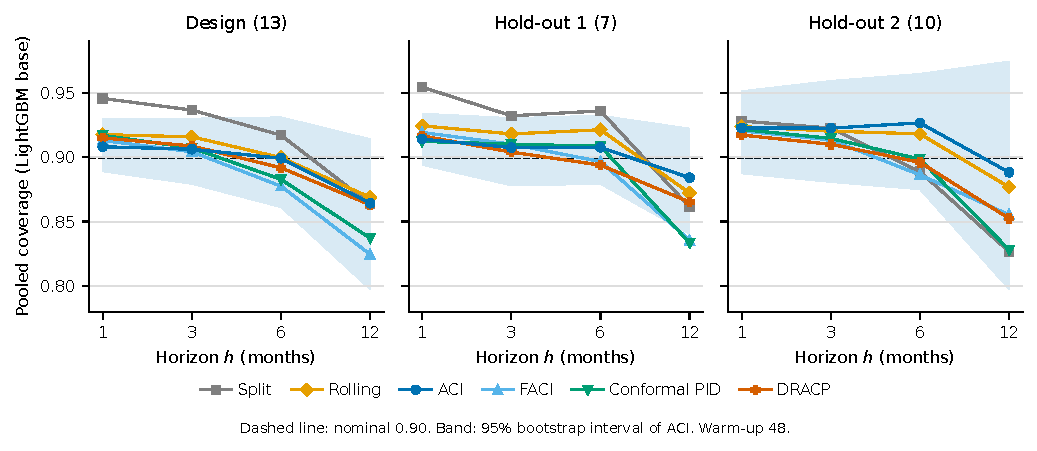
\includegraphics[width=\linewidth]{figures/fig_coverage_h.pdf}
\caption{Pooled empirical coverage by horizon and interval method for each panel (LightGBM base), against the nominal level 0.90.}
\label{fig:coverage_h}
\end{figure}

Tables~\ref{tab:ce_expl} and~\ref{tab:ce_ho1} give the calibration error. In the exploratory data the CE of ACI at $h=1,3,6,12$ is 0.013, 0.014, 0.035 and 0.069, against 0.038, 0.036, 0.050 and 0.091 for rolling and 0.071, 0.060, 0.069 and 0.139 for split. On the first hold-out panel it is 0.020, 0.020, 0.025 and 0.048 for ACI, 0.029, 0.036, 0.032 and 0.086 for rolling, and 0.056, 0.050, 0.053 and 0.119 for split.

\begin{table}[t]
\centering
\caption{Calibration error by base model, interval method and horizon, design panel (13 countries, exploratory, warm-up 48).}
\label{tab:ce_expl}
\small
\fittable{\begin{tabular}{llrrrr}
\toprule
Base model & Interval & $h{=}1$ & $h{=}3$ & $h{=}6$ & $h{=}12$ \\
\midrule
LightGBM & Split & 0.071 & 0.060 & 0.069 & 0.139 \\
 & Rolling & 0.038 & 0.036 & 0.050 & 0.091 \\
 & ACI & 0.013 & 0.014 & 0.035 & 0.069 \\
 & FACI & 0.014 & 0.018 & 0.041 & 0.101 \\
 & Conformal PID & 0.030 & 0.033 & 0.059 & 0.105 \\
 & DRACP & 0.016 & 0.016 & 0.033 & 0.074 \\
\midrule
ARIMA & Split & 0.064 & 0.064 & 0.098 & 0.148 \\
 & Rolling & 0.031 & 0.032 & 0.058 & 0.096 \\
 & ACI & 0.010 & 0.015 & 0.026 & 0.079 \\
 & FACI & 0.017 & 0.023 & 0.029 & 0.102 \\
 & Conformal PID & 0.027 & 0.020 & 0.046 & 0.099 \\
 & DRACP & 0.012 & 0.015 & 0.021 & 0.072 \\
 & Native & 0.047 & 0.066 & 0.089 & 0.137 \\
\midrule
Naive B & Split & 0.057 & 0.069 & 0.073 & 0.171 \\
 & Rolling & 0.031 & 0.035 & 0.043 & 0.100 \\
 & ACI & 0.012 & 0.016 & 0.024 & 0.057 \\
 & FACI & 0.017 & 0.018 & 0.039 & 0.124 \\
 & Conformal PID & 0.025 & 0.021 & 0.036 & 0.113 \\
 & DRACP & 0.017 & 0.017 & 0.028 & 0.071 \\
\midrule
ETS & Native & 0.044 & 0.051 & 0.064 & 0.116 \\
\bottomrule
\end{tabular}
}
\end{table}

\begin{table}[t]
\centering
\caption{Calibration error by base model, interval method and horizon, first hold-out panel (7 countries, warm-up 48).}
\label{tab:ce_ho1}
\small
\fittable{\begin{tabular}{llrrrr}
\toprule
Base model & Interval & $h{=}1$ & $h{=}3$ & $h{=}6$ & $h{=}12$ \\
\midrule
LightGBM & Split & 0.056 & 0.050 & 0.053 & 0.119 \\
 & Rolling & 0.029 & 0.036 & 0.032 & 0.086 \\
 & ACI & 0.020 & 0.020 & 0.025 & 0.048 \\
 & FACI & 0.023 & 0.023 & 0.013 & 0.070 \\
 & Conformal PID & 0.024 & 0.028 & 0.021 & 0.079 \\
 & DRACP & 0.021 & 0.019 & 0.022 & 0.047 \\
\midrule
ARIMA & Split & 0.067 & 0.065 & 0.061 & 0.106 \\
 & Rolling & 0.039 & 0.043 & 0.040 & 0.069 \\
 & ACI & 0.014 & 0.013 & 0.024 & 0.040 \\
 & FACI & 0.019 & 0.010 & 0.029 & 0.084 \\
 & Conformal PID & 0.029 & 0.037 & 0.034 & 0.083 \\
 & DRACP & 0.020 & 0.011 & 0.027 & 0.051 \\
 & Native & 0.053 & 0.058 & 0.062 & 0.073 \\
\midrule
Naive B & Split & 0.063 & 0.049 & 0.135 & 0.175 \\
 & Rolling & 0.039 & 0.030 & 0.061 & 0.052 \\
 & ACI & 0.015 & 0.021 & 0.030 & 0.032 \\
 & FACI & 0.026 & 0.020 & 0.036 & 0.079 \\
 & Conformal PID & 0.030 & 0.027 & 0.050 & 0.070 \\
 & DRACP & 0.024 & 0.024 & 0.032 & 0.055 \\
\midrule
ETS & Native & 0.056 & 0.035 & 0.048 & 0.053 \\
\bottomrule
\end{tabular}
}
\end{table}

The exploratory contrasts of the primary family at warm-up 48 are ACI minus rolling $-2.2$~pp at $h=3$ and $-1.5$~pp at $h=6$, with unadjusted $p$-values 0.030 and 0.020 but Holm-adjusted 0.090 and 0.078, so neither survives the family correction. ACI minus split (secondary) was $-4.6$~pp at $h=3$ (95\% interval \ci{-5.0}{-1.4}, unadjusted $p=0.001$) and $-3.4$~pp at $h=6$ ($p=0.0025$). DRACP minus ACI was $+0.2$~pp and $-0.2$~pp, within noise. Equivalence within 2~pp was shown at warm-up 48 (maximum one-sided $p$ 0.0085 and 0.0135) and not at warm-up 96 (0.128 and 0.146); at warm-up 96 DRACP was wider than ACI, with a Winkler score higher by 33.2 percent at $h=3$ (\ci{12.1}{75.9}, unadjusted $p=0.049$), so equivalence in the exploratory data is not stable across warm-ups. Per-country split coverage at $h=3$ ranges from 0.822 (Peru) to 1.000 (Indonesia), while ACI ranges from 0.886 to 0.934. At $h=12$ pooled coverage is below nominal for every method (0.825 to 0.869) and the adaptive methods do not repair it; the bootstrap intervals of ACI, DRACP, rolling and split include 0.90 (upper limits 0.915 to 0.920), those of FACI and conformal PID do not (0.876, 0.897). Mean absolute error relative to naive B was 0.74 (ARIMA), 0.72 (ETS) and 0.74 (LightGBM) at $h=3$ and 0.86, 0.93 and 0.91 at $h=12$.

\subsection{First hold-out panel and the decision rules R1--R5}\label{sec:holdout}

The hold-out run covers 7 countries and target months 2009-02 to 2026-06, with 205 and 199 pooled months at $h=3$ and $h=6$ in run A (warm-up 48) and 157 and 151 in run B (warm-up 96); run A has 1163, 1135, 1093 and 1009 unit-months at $h=1,3,6,12$. Pooled coverage in run A at $h=1,3,6,12$ is 0.954, 0.932, 0.936 and 0.861 for split, 0.924, 0.918, 0.921 and 0.872 for rolling, and 0.914, 0.907, 0.908 and 0.884 for ACI (all methods in the Appendix). At $h=12$ the pooled coverage of every method is below 0.90 (0.833 to 0.884); the bootstrap upper limits of ACI, DRACP, rolling and split (0.901 to 0.923) do not exclude 0.90, those of FACI and conformal PID (0.885, 0.884) do. Table~\ref{tab:contrasts} gives the primary contrasts of all panels, and the rules are applied as pre-specified.

\begin{table}[t]
\centering
\caption{Primary-family calibration-error contrasts by panel and base model: $T$ (pp of CE), 95\% block-bootstrap interval, Holm-adjusted $p$, minimum detectable difference (MDE) and verdict under the power rule. ``Inconclusive'' with an undefined MDE is not evidence of no effect.}
\label{tab:contrasts}
\small
\fittable{\begin{tabular}{llcllrrrl}
\toprule
Panel & Base & $h$ & Contrast & $T$ (pp) & 95\% CI & Holm $p$ & MDE (pp) & Verdict \\
\midrule
Design (13) & LightGBM & 3 & ACI $-$ rolling & $-$2.2 & [$-$2.7, +0.1] & 0.090 & -- & Inconclusive \\
 &  & 6 & ACI $-$ rolling & $-$1.5 & [$-$2.1, $-$0.1] & 0.078 & -- & Inconclusive \\
 &  & 3 & DRACP $-$ ACI & +0.2 & [$-$1.2, +1.0] & 1.000 & -- & Inconclusive \\
 &  & 6 & DRACP $-$ ACI & $-$0.2 & [$-$2.0, +1.3] & 1.000 & -- & Inconclusive \\
\midrule
Hold-out 1 (7) & LightGBM & 3 & ACI $-$ rolling & $-$1.6 & [$-$3.0, +0.5] & 0.350 & -- & Inconclusive \\
 &  & 6 & ACI $-$ rolling & $-$0.7 & [$-$2.8, +1.3] & 1.000 & -- & Inconclusive \\
 &  & 3 & DRACP $-$ ACI & $-$0.1 & [$-$1.2, +0.9] & 1.000 & -- & Inconclusive \\
 &  & 6 & DRACP $-$ ACI & $-$0.3 & [$-$1.4, +1.7] & 1.000 & -- & Inconclusive \\
\midrule
Design (13), from 2010 & LightGBM & 3 & ACI $-$ rolling & $-$2.1 & [$-$2.9, +0.5] & 0.216 & -- & Inconclusive \\
 &  & 6 & ACI $-$ rolling & $-$2.0 & [$-$3.1, +0.5] & 0.216 & -- & Inconclusive \\
 &  & 3 & DRACP $-$ ACI & $-$0.5 & [$-$1.6, +1.3] & 0.654 & -- & Inconclusive \\
 &  & 6 & DRACP $-$ ACI & +1.9 & [$-$1.0, +5.5] & 0.654 & -- & Inconclusive \\
\midrule
Design (13), from 2010 & Chronos & 3 & ACI $-$ rolling & $-$1.9 & [$-$2.3, +0.9] & 0.363 & -- & Inconclusive \\
 &  & 6 & ACI $-$ rolling & $-$2.0 & [$-$2.5, +0.8] & 0.358 & -- & Inconclusive \\
 &  & 3 & DRACP $-$ ACI & +0.0 & [$-$1.4, +1.3] & 0.982 & -- & Inconclusive \\
 &  & 6 & DRACP $-$ ACI & +2.4 & [$-$0.6, +5.9] & 0.363 & -- & Inconclusive \\
\midrule
Hold-out 1 (7), from 2010 & LightGBM & 3 & ACI $-$ rolling & $-$2.4 & [$-$5.5, +0.7] & 0.496 & -- & Inconclusive \\
 &  & 6 & ACI $-$ rolling & $-$4.7 & [$-$9.6, +0.5] & 0.390 & -- & Inconclusive \\
 &  & 3 & DRACP $-$ ACI & $-$0.8 & [$-$2.2, +1.2] & 0.656 & -- & Inconclusive \\
 &  & 6 & DRACP $-$ ACI & +0.2 & [$-$2.2, +1.4] & 0.904 & -- & Inconclusive \\
\midrule
Hold-out 1 (7), from 2010 & Chronos & 3 & ACI $-$ rolling & $-$1.3 & [$-$4.9, +0.7] & 1.000 & -- & Inconclusive \\
 &  & 6 & ACI $-$ rolling & $-$2.0 & [$-$4.5, +1.4] & 0.962 & -- & Inconclusive \\
 &  & 3 & DRACP $-$ ACI & $-$0.2 & [$-$2.0, +1.2] & 1.000 & -- & Inconclusive \\
 &  & 6 & DRACP $-$ ACI & +0.2 & [$-$2.5, +4.3] & 1.000 & -- & Inconclusive \\
\midrule
Hold-out 2 (10) & LightGBM & 3 & ACI $-$ rolling & $-$3.7 & [$-$5.1, $-$0.7] & 0.008 & 3.2 & Met \\
 &  & 6 & ACI $-$ rolling & $-$3.5 & [$-$4.9, +0.5] & 0.159 & 6.1 & Not met \\
 &  & 3 & DRACP $-$ ACI & $-$1.0 & [$-$2.0, +0.9] & 0.321 & -- & Inconclusive \\
 &  & 6 & DRACP $-$ ACI & $-$1.3 & [$-$2.7, +2.0] & 0.337 & -- & Inconclusive \\
\midrule
Hold-out 2 (10) & ARIMA & 3 & ACI $-$ rolling & $-$3.2 & [$-$3.6, $-$1.1] & 0.004 & 3.2 & Met \\
 &  & 6 & ACI $-$ rolling & $-$3.1 & [$-$3.9, $-$0.5] & 0.030 & 3.5 & Met \\
 &  & 3 & DRACP $-$ ACI & $-$1.5 & [$-$2.4, +0.8] & 0.199 & -- & Inconclusive \\
 &  & 6 & DRACP $-$ ACI & $-$1.8 & [$-$3.4, +0.7] & 0.199 & -- & Inconclusive \\
\midrule
Hold-out 2 (10) & Naive B & 3 & ACI $-$ rolling & $-$4.1 & [$-$4.9, $-$1.5] & 0.004 & 1.2 & Met \\
 &  & 6 & ACI $-$ rolling & $-$3.4 & [$-$4.7, $-$0.4] & 0.039 & 3.5 & Met \\
 &  & 3 & DRACP $-$ ACI & $-$1.2 & [$-$2.3, +0.9] & 0.422 & -- & Inconclusive \\
 &  & 6 & DRACP $-$ ACI & $-$1.8 & [$-$3.3, +2.5] & 0.422 & -- & Inconclusive \\
\midrule
Hold-out 2 (10) & Chronos & 3 & ACI $-$ rolling & $-$3.3 & [$-$4.0, $-$0.3] & 0.036 & -- & Inconclusive \\
 &  & 6 & ACI $-$ rolling & $-$2.5 & [$-$3.6, +0.1] & 0.088 & 6.6 & Not met \\
 &  & 3 & DRACP $-$ ACI & $-$0.5 & [$-$1.8, +1.3] & 0.454 & -- & Inconclusive \\
 &  & 6 & DRACP $-$ ACI & $-$1.2 & [$-$2.2, +1.3] & 0.443 & -- & Inconclusive \\
\bottomrule
\end{tabular}
}
\end{table}

\paragraph{R1 (ACI better calibrated than split): not met in the primary run; met at warm-up 96, a sensitivity run that is not promoted.} At warm-up 48 ACI minus split was $-3.0$~pp ($p=0.054$) at $h=3$ and $-2.8$~pp ($p=0.092$) at $h=6$, with intervals \ci{-5.4}{+0.5} and \ci{-3.9}{+1.2} that include zero; at warm-up 96 it was $-4.1$~pp ($p=0.018$) and $-5.9$~pp ($p=0.0025$). The direction replicates in both runs. Applying Holm over the two horizons (the result files have no Holm column for this secondary contrast) gives 0.108 at both horizons at warm-up 48 and 0.018 and 0.005 at warm-up 96; at warm-up 48 the rule fails with unadjusted as well as adjusted $p$-values, so the verdict for the primary configuration is ``not met'', and warm-up 96 was not promoted because R1 holds there.

\paragraph{R2 (ACI improves on rolling): not shown on this panel (MDE undefined, inconclusive).} Holm $p$ was 0.35 ($h=3$) and 1.0 ($h=6$) at warm-up 48 and 0.59 and 0.99 at warm-up 96, with point estimates $-1.6$ and $-0.7$~pp at warm-up 48. On the Winkler score ACI was 1.0 percent lower than rolling at $h=3$ (\ci{-7.1}{+4.1}) and 5.3 percent higher at $h=6$ (\ci{+1.4}{+8.1}, unadjusted $p=0.005$); these contrasts are descriptive. The second hold-out panel gives a different result (Section~\ref{sec:panel2}); the results are not combined.

\paragraph{R3 (DRACP against ACI): inconclusive.} Equivalence within 2~pp was shown at warm-up 48 (TOST $p$ 0.0005 at $h=3$ and 0.047 at $h=6$) and not at warm-up 96 (0.062 and 0.355). The wording ``no advantage, equivalent within 2~pp'' requires both warm-ups, so the verdict is inconclusive, and DRACP minus ACI is not negative with Holm $p$ below 0.05 at either warm-up, so ``DRACP better'' is not supported either. The 2~pp margin is of the size of the calibration error of ACI itself, so even the equivalence verdict at warm-up 48 is weak, and because the MDE of these contrasts is undefined, R5 classifies them as inconclusive whatever the TOST result.

\paragraph{R4 (delayed feedback explains the $h=12$ shortfall; ACI at least $+3$~pp): not met.} ACI coverage at $h=12$ was 0.884 delayed and 0.908 instant, a difference of $+2.4$~pp (Section~\ref{sec:feedback}).

\paragraph{R5 (power): all four primary contrasts are inconclusive.} The MDE is undefined on the full hold-out sample at both warm-ups, because the baseline calibration error is too small for a 10~pp improvement to be attainable. On random 15-month windows of the hold-out data the median MDE is 2.6 to 3.1~pp, but 63 to 68 percent of windows have an undefined MDE; it is also undefined in the exploratory data at warm-up 48. None of the four primary contrasts supports a conclusion.

\paragraph{What the hold-out result supports.} A direction in favour of adaptive methods over one-shot calibration, replicated in the exploratory data and at both warm-ups, with intervals that include zero at the primary warm-up. It does not support the statements that adaptivity helps beyond a rolling window or that DRACP is better than ACI. At $h=12$ the standard deviation of coverage across units is 0.058 for ACI and 0.152 for split.

\subsection{Robustness (S1, S2) and width}\label{sec:width}

The robustness analyses S1--S5 were written after the hold-out result and before they were computed, use only existing intervals and do not replace R1--R5. In S1 (leave one country out, LightGBM, warm-up 48; Appendix Table~\ref{tab:loo}) no removal flips the sign of ACI minus split in either sample (ranges $-5.1$ to $-2.1$~pp over both horizons and samples), so the advantage over a calibration done once does not depend on any single country. ACI minus rolling is negative for almost every removal (one flip in seven at $h=6$ on the hold-out panel, range $-1.3$ to $+0.1$~pp), but its interval includes zero in the primary run, so ``not shown'' stands. The DRACP minus ACI estimates sit at zero and change sign when one or two countries are removed. S2 (other base models; Appendix Table~\ref{tab:s2full}) is in Section~\ref{sec:basemodel}.

Three width statistics must be kept apart, and they do not give the same answer (Appendix Table~\ref{tab:width}). \emph{Median width relative to rolling:} at $h=1$ and $h=3$ ACI, DRACP and FACI have a lower median width in both samples (ACI 0.91 and 0.93 in the exploratory data, 0.84 and 0.90 on the first hold-out panel). \emph{Pooled mean width:} for ACI at $h=3$ it is larger than rolling's in both samples (4.28 against 3.95 exploratory, 5.856 against 5.786 hold-out), which indicates heavy tails in the adaptive widths; DRACP is wider than ACI at $h=3$ (4.97 against 4.28) and $h=12$ (24.3 against 15.5) in the exploratory data, but not on the hold-out panel, where its Winkler score at warm-up 96 was 5.8 percent lower than ACI's at $h=3$ (\ci{-14.2}{+3.3}, $p=0.18$). \emph{Winkler score:} the ratio to rolling for ACI, DRACP and FACI at $h=1$ and $h=3$ is 0.94 to 0.99 on the hold-out panel and 0.99 to 1.16 in the exploratory data (ACI 1.06 and DRACP 1.16 at $h=3$; ACI 6.3 percent higher than rolling at $h=3$, \ci{0.3}{19.4}, unadjusted $p=0.15$), and at $h=6$ and $h=12$ it exceeds 1 in most cells of both samples (up to 1.38). No efficiency advantage is established; at long horizons the better calibration is paid for with width or interval score.

\subsection{Second hold-out panel (extension)}\label{sec:panel2}

The second panel has 10 countries and 198 months from 2010-01 (89 and 83 pooled months at $h=3$ and $h=6$ at warm-up 48; 41 and 35 at warm-up 96), four base models and a Holm family of four tests per base model. Warm-up 48 is primary. Table~\ref{tab:ce_ho2} gives the CE: at $h=3$ and $h=6$ ACI has 0.033 and 0.045 for LightGBM, rolling 0.070 and 0.080, split 0.104 and 0.125, and the native ARIMA intervals 0.058 and 0.084. On the first hold-out panel the CE of the rolling window at $h=3$ and $h=6$ is 0.036 and 0.032, against 0.066 to 0.090 and 0.075 to 0.087 here; this is a descriptive observation, and its relation to the results below was not tested.

\begin{table}[t]
\centering
\caption{Calibration error by interval method, horizon and base model, second hold-out panel (10 countries, warm-up 48).}
\label{tab:ce_ho2}
\small
\fittable{\begin{tabular}{llrrrr}
\toprule
Base model & Interval & $h{=}1$ & $h{=}3$ & $h{=}6$ & $h{=}12$ \\
\midrule
LightGBM & Split & 0.084 & 0.104 & 0.125 & 0.154 \\
 & Rolling & 0.050 & 0.070 & 0.080 & 0.089 \\
 & ACI & 0.032 & 0.033 & 0.045 & 0.072 \\
 & FACI & 0.024 & 0.027 & 0.042 & 0.079 \\
 & Conformal PID & 0.043 & 0.051 & 0.070 & 0.103 \\
 & DRACP & 0.023 & 0.023 & 0.032 & 0.078 \\
\midrule
ARIMA & Split & 0.086 & 0.098 & 0.111 & 0.136 \\
 & Rolling & 0.053 & 0.066 & 0.084 & 0.089 \\
 & ACI & 0.026 & 0.034 & 0.052 & 0.074 \\
 & FACI & 0.033 & 0.023 & 0.035 & 0.075 \\
 & Conformal PID & 0.037 & 0.047 & 0.073 & 0.105 \\
 & DRACP & 0.017 & 0.019 & 0.034 & 0.071 \\
 & Native & 0.052 & 0.058 & 0.084 & 0.132 \\
\midrule
Naive B & Split & 0.079 & 0.122 & 0.105 & 0.188 \\
 & Rolling & 0.057 & 0.090 & 0.087 & 0.110 \\
 & ACI & 0.023 & 0.049 & 0.052 & 0.089 \\
 & FACI & 0.024 & 0.049 & 0.055 & 0.082 \\
 & Conformal PID & 0.054 & 0.073 & 0.074 & 0.122 \\
 & DRACP & 0.020 & 0.037 & 0.034 & 0.087 \\
\midrule
Chronos & Split & 0.078 & 0.109 & 0.107 & 0.111 \\
 & Rolling & 0.048 & 0.067 & 0.075 & 0.078 \\
 & ACI & 0.028 & 0.034 & 0.050 & 0.062 \\
 & FACI & 0.017 & 0.031 & 0.041 & 0.088 \\
 & Conformal PID & 0.040 & 0.052 & 0.073 & 0.105 \\
 & DRACP & 0.021 & 0.030 & 0.038 & 0.082 \\
\bottomrule
\end{tabular}
}
\end{table}

ACI minus split (secondary, $h=3$ and $h=6$) is $-7.0$ and $-8.0$~pp for LightGBM, $-6.4$ and $-5.8$ for ARIMA, $-7.3$ and $-5.3$ for naive B and $-7.4$ and $-5.7$ for Chronos (unadjusted $p\le 0.0045$). ACI with ARIMA has a lower CE than the native ARIMA intervals (0.034 against 0.058 at $h=3$, 0.052 against 0.084 at $h=6$); no interval for this contrast is reported for this panel.

\paragraph{R1.} At warm-up 48 R1 is met for all four base models at both horizons (unadjusted $p\le 0.0045$), by $-5.3$ to $-8.0$~pp. At warm-up 96 it is not met: LightGBM (0.048) and naive B (0.032) at $h=3$ have unadjusted $p$ below 0.05, all other cells are above, and with Holm over the two horizons none is below 0.05 (0.096 and 0.064). The direction replicates, and the threshold is met on this panel at warm-up 48 whereas on the first panel it was met only at warm-up 96.

\paragraph{R2: the result differs from the earlier panels.} At warm-up 48 R2 is met at $h=3$ for LightGBM, ARIMA and naive B (Holm 0.008, 0.004, 0.004) and at $h=6$ for ARIMA and naive B (0.030, 0.039). For Chronos at $h=3$ the Holm $p$ is 0.036 but the MDE is undefined, so under E5 that cell is inconclusive and is not counted as met; Chronos and LightGBM at $h=6$ are not met (0.088, 0.159). On the design and first hold-out panels it was not shown, with an undefined MDE (inconclusive). The earlier 20 countries re-run from 2010-01 give Holm $p$ of 0.22 to 1.0 with the MDE undefined in every cell, so those results are inconclusive under E5 and not evidence of no effect (Table~\ref{tab:contrasts}; Figure~\ref{fig:forest}). Three points should be read together. The point estimates are negative in every row; on the second panel they ($-2.5$ to $-4.1$~pp) are generally larger than on the earlier panels ($-0.7$ to $-2.4$~pp), with one exception (LightGBM on the re-run first panel at $h=6$: $-4.7$~pp, Holm $p=0.390$, \ci{-9.6}{+0.5}), so the direction does not differ between panels but its size and distance from the threshold do. ``ACI improves on a rolling window'' is reached under the pre-specified rule on one panel and not on the other two, and the data do not say why; candidate explanations (a shorter series, more volatile economies, a larger share of 198 months taken by the warm-up, a rolling window with a larger CE) were not tested. And the four base models share countries and months, so the three ``met'' cells at $h=3$ are not three independent confirmations. We do not average the panels and do not select the panel on which the rule is met.

\begin{figure}[t]
\centering
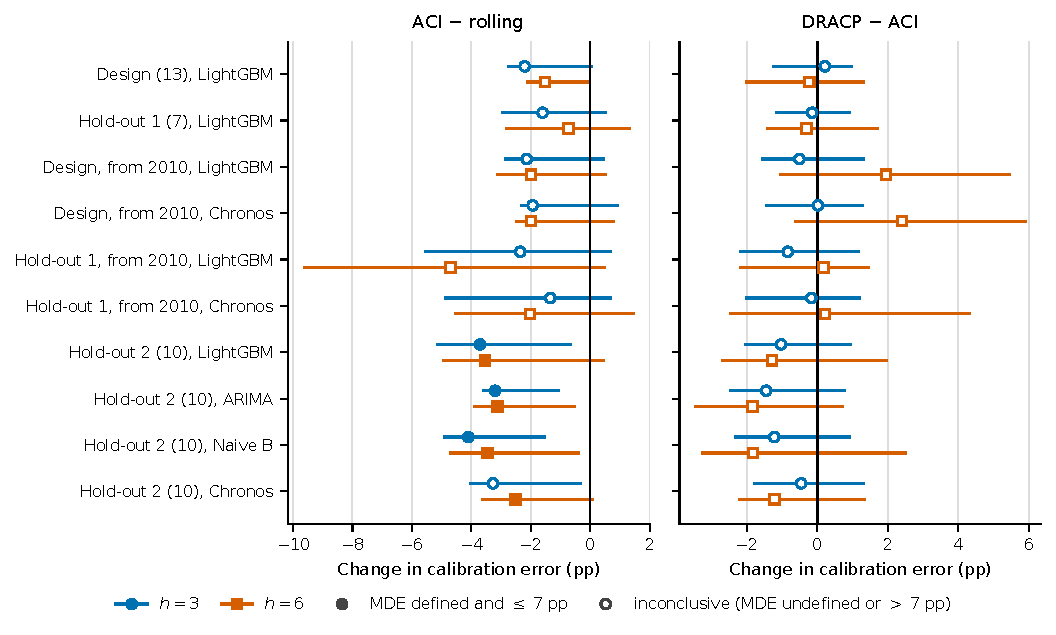
\includegraphics[width=\linewidth]{figures/fig_contrasts_forest.pdf}
\caption{Forest plot of the change in calibration error (pp) for ACI minus rolling and DRACP minus ACI, with 95\% block-bootstrap intervals. Contrasts with an undefined minimum detectable difference are inconclusive under rule E5 regardless of the interval. The panels are displayed side by side and not pooled.}
\label{fig:forest}
\end{figure}

\paragraph{Warm-up 96 shows nothing.} With 41 and 35 pooled months, ACI minus rolling is $-1.0$ to $-3.3$~pp at $h=3$ (Holm $p$ 0.147 to 1.0) and $+0.2$ (LightGBM), $+1.1$ (Chronos), $-0.5$ (ARIMA) and $-0.6$~pp (naive B) at $h=6$ (Holm $p\ge 0.59$), with the MDE undefined for every contrast; the run neither confirms nor contradicts the primary run and is not promoted.

\paragraph{R3 stays inconclusive.} At warm-up 48 DRACP has a lower CE than ACI in every cell, by 0.5 to 1.8~pp, and no difference has Holm $p$ below 0.05 (0.199 to 0.454). Equivalence within 2~pp holds only for Chronos at $h=3$ (TOST $p=0.0385$) and is not shown in the other seven cells ($p$ 0.15 to 0.76). At warm-up 96 equivalence holds for LightGBM and naive B at $h=3$ ($p=0.0375$ and 0.013) and not in the other six cells, and DRACP is better than ACI only at $h=6$ for naive B ($-2.3$~pp, Holm $p=0.002$). R3 requires the same verdict at both warm-ups, so it is not met, and under E5 every DRACP minus ACI contrast at warm-up 48 has an undefined MDE and is inconclusive whatever its $p$-value, including the equivalence of Chronos at $h=3$. The consistent tendency of DRACP towards a lower CE at warm-up 48 is a descriptive observation and not a result.

\paragraph{E5 and E2.} At warm-up 48 the MDE for ACI minus rolling is 3.2~pp ($h=3$) and 6.1~pp ($h=6$) for LightGBM, 3.2 and 3.5~pp for ARIMA, 1.2 and 3.5~pp for naive B, and 6.6~pp for Chronos at $h=6$ (undefined at $h=3$). Where R2 is not met (LightGBM and Chronos at $h=6$) the MDE of 6.1 and 6.6~pp exceeds the estimates, so ``not met'' is not evidence that the effect is absent. The conclusions about R1 and R3 do not depend on the base model, whereas the conclusion about R2 at $h=6$ does (met for ARIMA and naive B, not for LightGBM and Chronos). On the earlier 20 countries re-run from 2010-01 ACI minus split is $-3.5$ to $-9.4$~pp with unadjusted $p$ between 0.002 and 0.045. R4 was not part of the extension, and no instant-feedback run was made on the second panel.

\subsection{Ablations}\label{sec:ablation}

\paragraph{Base model.}\label{sec:basemodel} The contrasts were recomputed with ARIMA and naive B on the design and first hold-out panels (S2, Appendix Table~\ref{tab:s2full}), and Table~\ref{tab:ablation_base} gives the ablation on the second panel. ACI minus split is negative for all three base models in both samples (for naive B at $h=6$ on the first hold-out panel it is $-10.6$~pp). All DRACP minus ACI equivalence tests at warm-up 48 say ``equivalent'' within 2~pp except naive B at $h=6$ on the hold-out panel ($p=0.0515$), and at warm-up 96 on the hold-out panel most are ``not shown''. The direction ``ACI better than rolling'' holds for every base model and both samples, but unadjusted $p$-values range from 0.016 to 0.48 and none survives the correction of the pre-specified family.

\begin{table}[t]
\centering
\caption{Ablation over the base model on the second hold-out panel (warm-up 48): relative mean absolute error (naive B $=1$, all target months including flagged months), CE of ACI and of rolling, and ACI minus rolling in pp of CE with Holm $p$.}
\label{tab:ablation_base}
\small
\fittable{\begin{tabular}{lrrrrrrrr}
\toprule
& \multicolumn{2}{c}{Rel. MAE} & \multicolumn{2}{c}{CE, ACI} & \multicolumn{2}{c}{CE, rolling} & \multicolumn{2}{c}{ACI $-$ rolling, pp (Holm $p$)} \\
\cmidrule(lr){2-3}\cmidrule(lr){4-5}\cmidrule(lr){6-7}\cmidrule(lr){8-9}
Base model & $h{=}3$ & $h{=}6$ & $h{=}3$ & $h{=}6$ & $h{=}3$ & $h{=}6$ & $h{=}3$ & $h{=}6$ \\
\midrule
Naive B & 1.000 & 1.000 & 0.049 & 0.052 & 0.090 & 0.087 & $-$4.1 (0.004) & $-$3.4 (0.039) \\
ARIMA & 0.602 & 0.570 & 0.034 & 0.052 & 0.066 & 0.084 & $-$3.2 (0.004) & $-$3.1 (0.030) \\
LightGBM & 0.619 & 0.593 & 0.033 & 0.045 & 0.070 & 0.080 & $-$3.7 (0.008) & $-$3.5 (0.159) \\
Chronos & 0.586 & 0.581 & 0.034 & 0.050 & 0.067 & 0.075 & $-$3.3 (0.036) & $-$2.5 (0.088) \\
\bottomrule
\end{tabular}
}
\end{table}

\paragraph{Warm-up: 48 against 96.} Warm-up 96 is a sensitivity run applied to all methods and not promoted (Table~\ref{tab:ablation_warmup}). On the first hold-out panel ACI minus split moves from $-3.0$ and $-2.8$~pp at warm-up 48 to $-4.1$ and $-5.9$~pp at 96, which is what turns R1 from not met to met; ACI minus rolling is $-1.6$ and $-0.7$~pp at 48 and $-1.5$ and $-1.1$~pp at 96, with Holm $p$ 0.35 and 1.0 against 0.59 and 0.99. The larger warm-up removes target months (157 and 151 pooled months against 205 and 199), so the sample is also smaller, and on the second panel it leaves 41 and 35 months and shows nothing. The comparison does not select a configuration.

\begin{table}[t]
\centering
\caption{Ablation over the warm-up size: CE of ACI and rolling, ACI minus rolling and Holm $p$ at warm-up 48 (primary) and 96 (sensitivity, not promoted), by panel.}
\label{tab:ablation_warmup}
\small
\fittable{\begin{tabular}{llcrrrrrrrr}
\toprule
\multicolumn{3}{c}{} & \multicolumn{2}{c}{CE, ACI} & \multicolumn{2}{c}{CE, rolling} & \multicolumn{2}{c}{ACI $-$ rolling (pp)} & \multicolumn{2}{c}{Holm $p$} \\
\cmidrule(lr){4-5}\cmidrule(lr){6-7}\cmidrule(lr){8-9}\cmidrule(lr){10-11}
Panel & Base & $h$ & 48 & 96 & 48 & 96 & 48 & 96 & 48 & 96 \\
\midrule
Design (13) & LightGBM & 3 & 0.014 & 0.022 & 0.036 & 0.035 & $-$2.2 & $-$1.3 & 0.090 & 0.132 \\
 &  & 6 & 0.035 & 0.039 & 0.050 & 0.054 & $-$1.5 & $-$1.5 & 0.078 & 0.132 \\
\midrule
Hold-out 1 (7) & LightGBM & 3 & 0.020 & 0.027 & 0.036 & 0.042 & $-$1.6 & $-$1.5 & 0.350 & 0.592 \\
 &  & 6 & 0.025 & 0.030 & 0.032 & 0.041 & $-$0.7 & $-$1.1 & 1.000 & 0.990 \\
\midrule
Hold-out 2 (10) & LightGBM & 3 & 0.033 & 0.045 & 0.070 & 0.058 & $-$3.7 & $-$1.3 & 0.008 & 0.278 \\
 &  & 6 & 0.045 & 0.069 & 0.080 & 0.067 & $-$3.5 & +0.2 & 0.159 & 1.000 \\
\midrule
Hold-out 2 (10) & ARIMA & 3 & 0.034 & 0.043 & 0.066 & 0.053 & $-$3.2 & $-$1.0 & 0.004 & 0.340 \\
 &  & 6 & 0.052 & 0.081 & 0.084 & 0.086 & $-$3.1 & $-$0.5 & 0.030 & 0.682 \\
\midrule
Hold-out 2 (10) & Naive B & 3 & 0.049 & 0.050 & 0.090 & 0.083 & $-$4.1 & $-$3.3 & 0.004 & 0.147 \\
 &  & 6 & 0.052 & 0.071 & 0.087 & 0.077 & $-$3.4 & $-$0.6 & 0.039 & 0.593 \\
\midrule
Hold-out 2 (10) & Chronos & 3 & 0.034 & 0.048 & 0.067 & 0.063 & $-$3.3 & $-$1.5 & 0.036 & 1.000 \\
 &  & 6 & 0.050 & 0.084 & 0.075 & 0.073 & $-$2.5 & +1.1 & 0.088 & 1.000 \\
\bottomrule
\end{tabular}
}
\end{table}

\paragraph{Feedback delay.}\label{sec:feedback} At $h=12$ pooled coverage is below nominal for every method (0.83 to 0.88 on the first hold-out panel, 0.82 to 0.87 in the exploratory data), with the qualification on the bootstrap intervals given above. The diagnostic run releases each outcome at origin $+1$ instead of $+12$ (Table~\ref{tab:feedback}; paired block-bootstrap 95 percent intervals over the same cells). For ACI the change in coverage is $+4.1$~pp (\ci{1.4}{7.8}) in the exploratory data (1738 cells) and $+2.4$~pp (\ci{-0.1}{4.8}) on the hold-out panel (1009 cells); for DRACP $+4.3$ (\ci{1.4}{7.5}) and $+3.9$~pp (\ci{1.6}{6.4}); for FACI $+8.3$ (\ci{4.3}{13.6}) and $+6.4$~pp (\ci{2.5}{9.6}); for conformal PID $+5.1$ and $+5.3$~pp; for rolling $+1.3$~pp in both. R4 as pre-specified (ACI at least $+3$~pp) is not met: $+2.4$~pp, with an interval compatible with no effect and with an effect of about 5~pp. The supported statement is that delay accounts for part of the shortfall, with a size that depends on the method and sample; it is not shown that delay is, or is not, the main cause. The diagnostic is not a valid forecasting setup.

\begin{table}[t]
\centering
\caption{Ablation over the feedback delay (S3): coverage at $h=12$ with delayed and instant feedback, and the difference in pp with a 95\% paired block-bootstrap interval.}
\label{tab:feedback}
\small
\fittable{\begin{tabular}{lrrcrrc}
\toprule
& \multicolumn{3}{c}{Design (13), 1738 cells} & \multicolumn{3}{c}{Hold-out 1 (7), 1009 cells} \\
\cmidrule(lr){2-4}\cmidrule(lr){5-7}
Method & Delayed & Instant & Diff. (pp) [95\% CI] & Delayed & Instant & Diff. (pp) [95\% CI] \\
\midrule
Split & 0.864 & 0.864 & +0.0 [+0.0, +0.0] & 0.861 & 0.861 & +0.0 [+0.0, +0.0] \\
Rolling & 0.869 & 0.882 & +1.3 [+0.2, +3.1] & 0.872 & 0.885 & +1.3 [+0.1, +1.7] \\
ACI & 0.864 & 0.905 & +4.1 [+1.4, +7.8] & 0.884 & 0.908 & +2.4 [$-$0.1, +4.8] \\
FACI & 0.825 & 0.907 & +8.3 [+4.3, +13.6] & 0.835 & 0.900 & +6.4 [+2.5, +9.6] \\
Conformal PID & 0.837 & 0.888 & +5.1 [+2.0, +9.0] & 0.833 & 0.886 & +5.3 [+2.5, +7.9] \\
DRACP & 0.863 & 0.906 & +4.3 [+1.4, +7.5] & 0.865 & 0.904 & +3.9 [+1.6, +6.4] \\
\bottomrule
\end{tabular}
}
\end{table}

\paragraph{Native intervals against conformal calibration.}\label{sec:native} The analysis S7 compares conformal calibration with the native intervals of ARIMA (Gaussian) and ETS (simulated). It is post hoc, secondary, without multiplicity correction, with unadjusted descriptive $p$-values; ETS has no conformal version in the engine, so only its native CE is reported (Table~\ref{tab:native}). In the exploratory data the native ARIMA intervals have a CE of 0.047, 0.066, 0.089 and 0.137 at $h=1,3,6,12$ against 0.010, 0.015, 0.026 and 0.079 for ARIMA with ACI, and native ETS is of the same order as native ARIMA in both samples. The contrast ACI minus native with ARIMA is $-3.7$, $-5.1$, $-6.4$ and $-5.8$~pp in the exploratory data and $-3.9$, $-4.5$, $-3.8$ and $-3.3$~pp on the hold-out panel (unadjusted $p$ below 0.001, 0.010, 0.082 and 0.100). ACI gives a lower CE than the native ARIMA intervals at every horizon in both samples, by about 3 to 6~pp; on the hold-out panel the interval excludes zero at $h=1$ and $h=3$ and includes it at $h=6$ and $h=12$. The mean coverage of native ARIMA intervals looks acceptable on the hold-out panel (0.943, 0.930, 0.919, 0.885 at $h=1,3,6,12$) because over-coverage in some countries offsets under-coverage in others. The evidence is weaker in procedure than that for the pre-specified contrasts, although its direction is consistent.

\begin{table}[t]
\centering
\caption{Ablation over the reference interval (S7, post hoc): CE of native ARIMA and ETS intervals and of ARIMA with ACI, and the contrast ACI minus native (pp of CE, 95\% interval, unadjusted $p$).}
\label{tab:native}
\small
\fittable{\begin{tabular}{lcrrrcr}
\toprule
Panel & $h$ & ARIMA native & ARIMA + ACI & ETS native & ACI $-$ native, pp [95\% CI] & $p$ \\
\midrule
Design (13) & 1 & 0.047 & 0.010 & 0.044 & $-$3.7 [$-$4.6, $-$0.6] & 0.004 \\
 & 3 & 0.066 & 0.015 & 0.051 & $-$5.1 [$-$6.2, $-$1.0] & 0.003 \\
 & 6 & 0.089 & 0.026 & 0.064 & $-$6.4 [$-$7.7, $-$1.3] & 0.002 \\
 & 12 & 0.137 & 0.079 & 0.116 & $-$5.8 [$-$7.8, $-$1.9] & 0.003 \\
\midrule
Hold-out 1 (7) & 1 & 0.053 & 0.014 & 0.056 & $-$3.9 [$-$4.5, $-$1.3] & $<$0.001 \\
 & 3 & 0.058 & 0.013 & 0.035 & $-$4.5 [$-$4.8, $-$0.6] & 0.010 \\
 & 6 & 0.062 & 0.024 & 0.048 & $-$3.8 [$-$4.4, +1.2] & 0.082 \\
 & 12 & 0.073 & 0.040 & 0.053 & $-$3.3 [$-$4.9, +1.3] & 0.100 \\
\midrule
Hold-out 2 (10) & 1 & 0.052 & 0.026 & -- & -- & -- \\
 & 3 & 0.058 & 0.034 & -- & -- & -- \\
 & 6 & 0.084 & 0.052 & -- & -- & -- \\
 & 12 & 0.132 & 0.074 & -- & -- & -- \\
\bottomrule
\end{tabular}
}
\end{table}

\paragraph{Point accuracy of Chronos.}\label{sec:chronos} Months before 2025-01 are flagged \texttt{possibly\_seen}. Over all target months of the second panel at warm-up 48 (naive B $=1$) the relative MAE is 0.737, 0.586, 0.581 and 0.934 for Chronos at $h=1,3,6,12$, against 0.779, 0.602, 0.570 and 0.880 for ARIMA and 0.817, 0.619, 0.593 and 0.943 for LightGBM; this comparison includes months on which Chronos may have an unfair advantage and supports no claim. Following E4, accuracy claims use only the 22 clean calendar months from 2025-01 (567 country-month cells per horizon, 30 countries). Table~\ref{tab:chronos_mae} and Figure~\ref{fig:chronos} give relative MAE and the paired difference in MAE (Chronos minus the other model, pp; negative favours Chronos) with a block-bootstrap interval (blocks of 3 months, months resampled jointly); intervals are unadjusted and descriptive. The relative MAE of Chronos is 0.774, 0.699, 0.654 and 0.895 at $h=1,3,6,12$ (LightGBM 0.824 to 0.995; ARIMA 0.700 to 0.905). Against LightGBM the interval excludes zero at $h=1$, 6 and 12 and against ARIMA at $h=1$ and 3 (at $h=6$ the upper limit is $+0.002$); against naive B it excludes zero at every horizon; no interval favours LightGBM or ARIMA over Chronos. Chronos was at least as accurate as LightGBM and ARIMA in this period and more accurate than the naive baseline. The sample is thin, the block length short, the leakage assumption unverified, and the results are descriptive and not a ranking of forecasters; calibration contrasts for Chronos use all months with the flag.

\begin{table}[t]
\centering
\caption{Point accuracy of Chronos on the clean target months from 2025-01 (22 months, 30 countries): MAE relative to naive B, and difference in MAE with a paired block-bootstrap 95\% interval (pp; negative favours Chronos).}
\label{tab:chronos_mae}
\small
\fittable{\begin{tabular}{crrrccc}
\toprule
& \multicolumn{3}{c}{Relative MAE (naive B $=1$)} & \multicolumn{3}{c}{MAE difference, Chronos $-$ other (pp)} \\
\cmidrule(lr){2-4}\cmidrule(lr){5-7}
$h$ & Chronos & LightGBM & ARIMA & vs LightGBM & vs ARIMA & vs naive B \\
\midrule
1 & 0.774 & 0.824 & 0.854 & $-$0.023 [$-$0.047, $-$0.007] & $-$0.037 [$-$0.053, $-$0.021] & $-$0.104 [$-$0.134, $-$0.081] \\
3 & 0.699 & 0.725 & 0.773 & $-$0.031 [$-$0.078, +0.036] & $-$0.086 [$-$0.139, $-$0.031] & $-$0.350 [$-$0.519, $-$0.206] \\
6 & 0.654 & 0.694 & 0.700 & $-$0.084 [$-$0.129, $-$0.025] & $-$0.097 [$-$0.204, +0.002] & $-$0.720 [$-$0.905, $-$0.527] \\
12 & 0.895 & 0.995 & 0.905 & $-$0.245 [$-$0.465, $-$0.019] & $-$0.024 [$-$0.122, +0.139] & $-$0.256 [$-$0.449, $-$0.041] \\
\bottomrule
\end{tabular}
}
\end{table}

\begin{figure}[t]
\centering
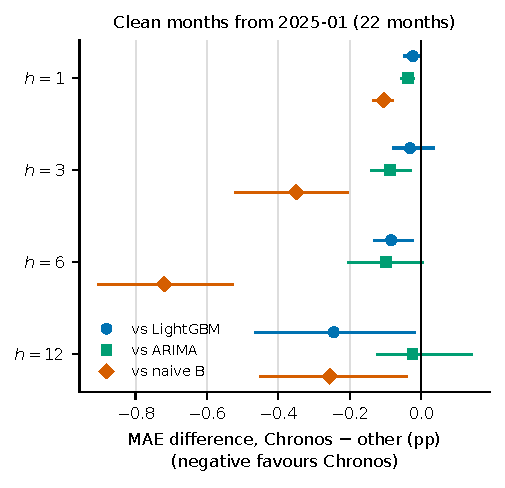
\includegraphics[width=\linewidth]{figures/fig_chronos_accuracy.pdf}
\caption{Point accuracy of Chronos relative to the other forecasters by horizon. Claims are limited to the 22 target months from 2025-01; earlier months are flagged as possibly seen in pretraining.}
\label{fig:chronos}
\end{figure}

\subsection{Other analyses}\label{sec:other}

\paragraph{Post-2025-06 months of the 13 countries (not used).} The run evaluating the design countries on target months from 2025-07 has eleven contributing countries (Nigeria ends in 2024-12 because of the CPI break; Russia has no usable stretch after 2022-03), each with at most 16 months. With blocks of 12 it is degenerate (confidence limits coincide with the estimate, $p$-values sit at the resampling floor) and is not used for any claim; pooled ACI coverage is 0.904, 0.922 and 0.940 at $h=1,3,6$, and no conclusion is drawn.

\paragraph{Exploratory stress and Kazakhstan.} The secondary exchange-rate stress analysis (exploratory sample only; top-decile coverage of ACI 0.849 at $h=3$ against about 0.87 to 0.98 in other deciles, roughly two standard errors, non-monotone) and the post hoc descriptive analysis of Kazakhstan alone (S6, one design country with about 137 origins; no mechanism isolated) are documented in the repository and not repeated here; no stress result exists for the hold-out panels and no confirmatory claim about stress or Kazakhstan is made.

\section{Discussion}\label{sec:discussion}

\paragraph{What is established.} Four statements are supported, with qualifications. First, adaptive conformal intervals were better calibrated than a calibration performed once and never updated; the direction is the same in the exploratory data, on the first hold-out panel at both warm-ups, for three base forecasters and after removing any single country, but R1 was met on that panel only at warm-up 96, a sensitivity run, and at warm-up 48 the intervals include zero (\ci{-5.4}{+0.5} and \ci{-3.9}{+1.2}). The statement is one of consistent direction, not of a pre-specified confirmation on that panel; on the second panel R1 was met at warm-up 48 for all four base models and not at 96. Second, in a secondary post hoc analysis ACI with ARIMA had a lower CE than the native ARIMA intervals at every horizon in both samples (the interval includes zero at $h=6$ and $h=12$ on the first hold-out panel). Third, at 12 months pooled coverage is below nominal for every method on the design and first hold-out panels, and delayed feedback explains part of the shortfall, by an amount that depends on method and sample. Fourth, ACI, DRACP and FACI have a median width below rolling at short horizons, but the pooled mean width of ACI at $h=3$ exceeds rolling's in both samples and the Winkler ratio is below 1 only on the hold-out panel at $h=1$ and $h=3$ (0.95 and 0.99 for ACI, the latter with an interval that includes zero); no efficiency advantage is established.

\paragraph{What is not established.} (i) Whether ACI improves on a rolling window depends on the panel: not shown on the design and first hold-out panels (point estimates of about 1 to 3~pp in the direction of an advantage, MDE undefined, inconclusive), not significant on the earlier 20 countries re-run from 2010-01 (Holm $p$ 0.22 to 1.0, MDE undefined, inconclusive under E5), and met at warm-up 48 on the second panel at $h=3$ for LightGBM, ARIMA and naive B and at $h=6$ for ARIMA and naive B, but inconclusive for Chronos at $h=3$ and not met for Chronos and LightGBM at $h=6$. The reason is unknown; the supported statement is that the result is panel dependent, and it is neither ``ACI does not improve on a rolling window'' nor ``ACI improves on a rolling window''. (ii) An advantage of DRACP over ACI was not detected and equivalence was not stable across warm-ups (R3); on the second panel DRACP had a lower CE in every cell at warm-up 48, by 0.5 to 1.8~pp, with no Holm $p$ below 0.05. (iii) That delay explains the $h=12$ shortfall was not met at the threshold (R4). None of these is evidence that the effects are absent; ``DRACP does not transfer'' and ``ACI and DRACP are equal'' are not allowed by the data.

\paragraph{Why null results.} The data do not apportion the reasons. The first hold-out panel has 7 countries and about 200 origin months at $h=3$, errors of $h$-step forecasts overlap, adaptive methods have a memory of about 50 months, and countries share shocks, so the block-bootstrap intervals are about 2 to 6~pp wide. There is a ceiling effect: the CE of rolling on that panel is already small (0.029, 0.036, 0.032 at $h=1,3,6$ against 0.020, 0.020, 0.025 for ACI), the power simulation cannot create an improvement larger than the baseline CE, and 80 percent power was not reached up to 10~pp, so we read the undefined MDE as a limit of the design and not as a finding about the methods. The 2~pp margin is about the size of ACI's own CE, so ``equivalent'' is weak by construction and the null outcomes against ACI were likely before the run; the informative contrasts are those against weak references, split (CE 0.050 to 0.056) and the native intervals. A true small difference cannot be separated from low power. For DRACP, regime and scale models are trained on half of the warm-up (24 rows at warm-up 48), its results depend on the warm-up, and its authors state that its advantage is specific to one-step-ahead forecasting, which our multi-month design does not test; our partial one-step reproduction could not distinguish ACI and DRACP either.

\paragraph{The panel dependence of R2.} The second panel is a counter-example to the null outcomes and is reported beside them. Candidate explanations are a shorter series, lower-income and more volatile economies, a warm-up occupying a larger share of 198 months, and a rolling window with a larger CE (0.066 to 0.090 at $h=3$ against 0.036 on the first panel; the MDE is defined here, 1.2 to 6.6~pp, which is consistent with the ceiling argument), but none was tested and warm-up 96 cannot arbitrate. The panels are not averaged and the favourable panel is not selected; a reader who wants a recommendation for a new set of countries cannot take it from this study.

\paragraph{Calibrated is not useful, and practice.} A nominal-coverage interval can be very wide: the pooled mean width of ACI is 4.28 pp at $h=3$ and 15.5 at $h=12$ in the exploratory data, and at $h=12$ an interval with honest 90 percent coverage may be too wide for practical use. A practitioner should not calibrate once and leave the calibration unchanged: one-shot calibration had a higher CE than ACI in every reported contrast for LightGBM, ARIMA and naive B and for Chronos in all but one cell (second panel, warm-up 96, $h=6$, $+0.8$~pp, indistinguishable from zero), and its coverage varied most across countries (standard deviation at $h=12$ 0.152 for split against 0.058 for ACI), although R1 was met on the first panel only at the sensitivity warm-up. Between a rolling window and ACI the study cannot recommend one on statistical or efficiency grounds. At 12 months users should treat the nominal level as an upper bound, since part of the shortfall comes from the delay in outcomes and cannot be removed in real use. The hold-out countries share calendar months with the design sample, so agreement between samples is weaker evidence of generality than if they had been observed in other periods.

\section{Limitations}\label{sec:limitations}

All 21 limitations of the full version are kept, grouped; the bracketed numbers give their order in the full version.

\paragraph{Design and inference.}
\begin{itemize}
\item[(1, 20)] The hold-out countries are untouched with respect to countries only and share calendar months with the design sample. Methods, contrasts, horizons, the 2~pp margin and the 3~pp and 7~pp thresholds were chosen on the design countries, and R1--R5 were written after the exploratory results were known. Pre-specification is a self-attested commit history of one author (all entries on 2026-11-18 or 2026-11-19), not an external registry. The extension rules E1--E5 were written knowing every earlier result, so it is a replication on new countries and not a blind test.
\item[(2, 9)] The MDE is undefined on the full first hold-out sample for all four primary contrasts, so null outcomes are inconclusive and not evidence of equality; the 2~pp margin is about the size of ACI's own CE, so equivalence is weak by construction. The MDE simulation is not independently reviewed and assumes that the observed hit pattern describes the true dependence. CE is biased upward in small samples, the validity of its bootstrap at the boundary of the absolute value was not checked by simulation, and the 2~pp margin and the 3~pp threshold of R4 are not justified beyond being fixed in advance.
\item[(15)] The post hoc additions have no multiplicity correction: S6 is descriptive for one design country with about 137 origins, and S7 uses unadjusted $p$-values and one base model for the contrast.
\end{itemize}

\paragraph{Data and panels.}
\begin{itemize}
\item[(3, 12, 17)] The first hold-out panel has 7 countries, with high-inflation episodes in Ghana and Angola, so pooled results can be driven by few units (removing one country flips ACI against rolling at $h=6$ in one case of seven). The post-2025-06 months of the design countries are degenerate and unused, and $h=12$ has few non-overlapping windows (80 on the first panel). The second panel has 198 months (89 and 83 pooled months at warm-up 48, 41 and 35 at 96, where it shows nothing), the MDE is undefined for every contrast at warm-up 96 and every DRACP minus ACI contrast at 48, and several of its countries failed the first hold-out rule on history length.
\item[(5, 7)] Data vintages were not checked although the IMF publishes them; evaluation uses revised data of the snapshot date, and Nigeria ends at 2024-12 because of a methodology break. ``Commodity-dependent'' has no measurable criterion (no export-share rule; Georgia and Uruguay are borderline), and the hold-out sets follow IMF data availability.
\item[(10, 11)] The exchange-rate stress analysis is secondary and exploratory: the flag is a weak proxy for inflation shocks (lift below 2), many deciles, methods and horizons were examined, and pegged and managed currencies were not separated. The protocol mentions a central-bank-target baseline, an exchange-rate-regime split and per-country heterogeneity beyond coverage ranges, which the results do not report; native intervals and Kazakhstan are reported only post hoc or descriptively.
\end{itemize}

\paragraph{Methods and literature.}
\begin{itemize}
\item[(4, 14)] LightGBM is the base model of the decision rules; ARIMA and naive B give the same direction but were not part of them. The four extension base models share countries and months and are not independent replications, with Holm applied within each. Hyperparameters were fixed in advance, the point models are simple, and better forecasts could change absolute calibration and width.
\item[(8, 6)] The reproduction of DRACP is partial (five countries, one seed, ACI 0.874 and DRACP 0.871 against 0.884 and 0.890 over 48 series and 20 seeds; a published number within 2~pp could not be tested because the published figures average different series). The configuration follows the reproduction script and was not tuned, and the description of DRACP is as given by its authors. No systematic literature search was run, so statements about novelty rest on the author's reading, and several bibliography entries need verification.
\item[(13)] The platform uses a different point forecast and a smaller minimum calibration size, so the benchmark applies to its interval method only; it is an engineering application.
\end{itemize}

\paragraph{Extension and interpretation.}
\begin{itemize}
\item[(16)] The ACI-against-rolling result depends on the panel and the reason is unknown: R2 is met at warm-up 48 on the second panel (at $h=3$ for LightGBM, ARIMA and naive B, Holm 0.008, 0.004, 0.004; at $h=6$ for ARIMA and naive B, 0.030, 0.039; Chronos at $h=3$ has an undefined MDE and is inconclusive under E5), not shown (inconclusive) on the design and first panels, and not significant (inconclusive) on the earlier 20 countries re-run from 2010-01. Candidate explanations were not tested; the panels are not pooled and none is selected.
\item[(18)] Chronos may have seen public CPI series in pretraining; the cutoff was not verified and 2025-01 is a conservative assumption. Accuracy claims rest on 22 months (567 cells per horizon) with a short block length, calibration contrasts for Chronos use all months with the flag, only the smallest Chronos-Bolt model was used zero-shot, and on the earlier 20 countries contrasts were analysed only for LightGBM and Chronos, which narrows the E-B analysis of the protocol.
\item[(19)] \ExplainerStatus{} The 468-prompt, two-condition evaluation (936 calls) is specified; the output of the fake client used to test the code is not a result.
\item[(21)] Calibrated does not mean useful: the pooled mean width of ACI is 4.28 pp at $h=3$ and 15.5 at $h=12$ in the exploratory data, so better calibration at long horizons is paid for in width or interval score, and no width at which an interval becomes useful is established or compared with a decision-relevant threshold.
\end{itemize}

\section{Conclusion}\label{sec:conclusion}

We benchmarked split, rolling, ACI, FACI, conformal PID and DRACP prediction intervals for the cumulative log growth of the consumer price index at horizons of 1 to 12 months on 30 economies in three panels, with four base forecasters including a zero-shot foundation model, and with decision rules fixed in a version-controlled protocol before the hold-out runs. The pre-specification is a self-attested commit history, and the rules were written after the exploratory results were known.

Three findings are supported. Adaptive methods had a lower calibration error than a calibration performed once and, in a post hoc comparison restricted to ARIMA, than the native intervals of that model, with a direction consistent across samples, base models and warm-ups (one cell, Chronos at $h=6$ and warm-up 96 on the second hold-out panel, has the opposite sign), although the pre-specified rule R1 was met on the first hold-out panel only at the 96-month sensitivity warm-up and the primary-warm-up intervals include zero. At 12 months pooled coverage is below nominal for every method on the design and first hold-out panels, and delayed feedback explains part of the shortfall by an amount that did not reach the pre-specified threshold. And whether adaptivity helps beyond a rolling window has no panel-independent answer: it was not shown on two panels and was met under the pre-specified rule in part of the cells of a third, for unknown reasons.

Several findings are not established. No advantage of DRACP over ACI was detected, equivalence within 2~pp was not stable across warm-ups, and the margin is about the size of ACI's own calibration error, so the verdict is weak by construction. No efficiency advantage in width or interval score is established, and calibrated intervals are not thereby useful ones. The accuracy of Chronos on the 22 target months from 2025-01 was descriptively at least that of LightGBM and ARIMA, under an unverified assumption about its pretraining cutoff. \ExplainerStatus{}

The paper is a controlled transfer and benchmark study and claims nothing beyond that. Its null and inconclusive outcomes come from a design whose reference methods were already well calibrated and whose power was limited, and they are not evidence of equality. The next steps are to add countries and periods so that power is defined for the contrasts against ACI, to test the candidate explanations for the panel dependence, and to examine interval width against decision-relevant thresholds.

\section{Reproducibility and availability}\label{sec:repro}

The work is in the EVision project repository: the protocol with its change log, the shock definition and the results documents (\texttt{docs/thesis/}); small CSV result tables per run (\texttt{docs/thesis/results/}); the Node data-download scripts, the dated hashed snapshots and the experiment engine with its tests (\texttt{scripts/thesis/}); the platform and explanation services (\texttt{backend/fastapi\_service/}); and the full paper with its build instructions (\texttt{paper/}). The commit hashes of each protocol step, the SHA-256 hashes of the four data snapshots, the per-check robustness tables (S4, S5), the shock-rule validity checks, the Kazakhstan analysis and the exact command lines are in the repository documents and in the full version of this paper, and are omitted here. The command lines of the sensitivity run on the design countries, of the instant-feedback diagnostic on the design countries and of the extension runs were reconstructed from the command-line options and run names and are not recorded verbatim; they are to be verified before submission.

The engine runs in a Python 3.12 virtual environment (pandas, numpy, scipy, statsmodels, scikit-learn, LightGBM and the \texttt{dracp} package, version 0.2.0 in the reproduction check; the Chronos package version is not recorded and is to be verified). Its 81 tests cover data chaining, the absence of look-ahead in the forecasters, the timing of delayed and instant feedback, the equivalence of the independent ACI implementation with the package at $h=1$, calibration-error contrasts, Holm, TOST, the power simulation, the hold-out loader, the robustness analyses, the Chronos forecaster with its leakage flag and the reading of results files. The figures and tables are generated from the committed result files by \texttt{scripts/thesis/paper/build\_paper\_assets.py}; numbers in the running text were taken from the project manuscript and result documents. The underlying series are public IMF data, and no private data are used.


\bibliographystyle{plainnat}
\bibliography{references}

\appendix
\section{Stable robustness tables}\label{app:extra}

Further per-check detail (the S4 and S5 tables, the shock-rule validity checks, the Kazakhstan analysis, the protocol change log with commit hashes, the data snapshot hashes and the reproduction commands) is in the repository and in the full version of this paper.

\begin{table}[H]
\centering
\caption{S1: range of the contrast over leave-one-country-out removals (pp of CE) and number of sign flips of the full-sample estimate.}
\label{tab:loo}
\small
\begin{tabular}{@{}lll@{}}
\toprule
Contrast, horizon & Exploratory (13 countries) & First hold-out (7 countries) \\
\midrule
ACI $-$ split, $h=3$ & $-5.1$ to $-4.2$, 0 flips & $-4.1$ to $-2.2$, 0 flips \\
ACI $-$ split, $h=6$ & $-4.1$ to $-2.5$, 0 flips & $-3.5$ to $-2.1$, 0 flips \\
ACI $-$ rolling, $h=3$ & $-2.5$ to $-1.8$, 0 flips & $-2.2$ to $-1.0$, 0 flips \\
ACI $-$ rolling, $h=6$ & $-1.7$ to $-1.3$, 0 flips & $-1.3$ to $+0.1$, 1 of 7 flips \\
DRACP $-$ ACI, $h=3$ & $0.0$ to $+0.4$, 0 flips & $-0.4$ to $-0.1$, 0 flips \\
DRACP $-$ ACI, $h=6$ & $-0.5$ to $+0.1$, 2 of 13 flips & $-0.7$ to $+0.1$, 1 of 7 flips \\
\bottomrule
\end{tabular}
\end{table}

\begin{table}[H]
\centering
\caption{S2 (other base models): ACI minus rolling and DRACP minus ACI by base model (pp of CE; unadjusted bootstrap $p$ in parentheses).}
\label{tab:s2full}
\small
\begin{tabular}{@{}llccc@{}}
\toprule
Sample & Contrast, horizon & LightGBM & ARIMA & Naive B \\
\midrule
Exploratory & ACI $-$ rolling, 3 & $-2.2$ (0.030) & $-1.7$ (0.059) & $-1.9$ (0.053) \\
Exploratory & ACI $-$ rolling, 6 & $-1.5$ (0.020) & $-3.3$ (0.016) & $-1.9$ (0.067) \\
Exploratory & DRACP $-$ ACI, 3 & $+0.2$ (0.70) & $+0.0$ (0.98) & $+0.1$ (0.82) \\
Exploratory & DRACP $-$ ACI, 6 & $-0.2$ (0.78) & $-0.4$ (0.54) & $+0.4$ (0.54) \\
Hold-out & ACI $-$ rolling, 3 & $-1.6$ (0.087) & $-3.0$ (0.030) & $-0.9$ (0.22) \\
Hold-out & ACI $-$ rolling, 6 & $-0.7$ (0.48) & $-1.6$ (0.21) & $-3.2$ (0.053) \\
Hold-out & DRACP $-$ ACI, 3 & $-0.1$ (0.76) & $-0.2$ (0.80) & $+0.2$ (0.71) \\
Hold-out & DRACP $-$ ACI, 6 & $-0.3$ (0.66) & $+0.2$ (0.79) & $+0.3$ (0.75) \\
\bottomrule
\end{tabular}
\end{table}

\begin{table}[H]
\centering
\caption{Calibration error / Winkler ratio / median width ratio relative to rolling conformal, by panel, interval method and horizon (LightGBM, warm-up 48; a ratio below 1 is better than rolling).}
\label{tab:width}
\small
\fittable{\begin{tabular}{lcccc}
\toprule
Method & $h{=}1$ & $h{=}3$ & $h{=}6$ & $h{=}12$ \\
\midrule
\multicolumn{5}{l}{\emph{Design (13), warm-up 48}} \\
ACI & 0.013 / 0.99 / 0.91 & 0.014 / 1.06 / 0.93 & 0.035 / 1.21 / 1.11 & 0.069 / 1.00 / 1.03 \\
DRACP & 0.016 / 1.07 / 0.95 & 0.016 / 1.16 / 0.95 & 0.033 / 1.21 / 1.09 & 0.074 / 1.38 / 1.69 \\
FACI & 0.014 / 1.00 / 0.95 & 0.018 / 1.05 / 0.94 & 0.041 / 1.06 / 0.88 & 0.101 / 0.96 / 0.91 \\
Conformal PID & 0.030 / 1.00 / 0.96 & 0.033 / 1.02 / 0.98 & 0.059 / 1.02 / 0.94 & 0.105 / 1.01 / 1.01 \\
Rolling & 0.038 / 1.00 / 1.00 & 0.036 / 1.00 / 1.00 & 0.050 / 1.00 / 1.00 & 0.091 / 1.00 / 1.00 \\
Split & 0.071 / 1.08 / 1.24 & 0.060 / 1.11 / 1.29 & 0.069 / 1.02 / 1.13 & 0.139 / 0.93 / 0.94 \\
\midrule
\multicolumn{5}{l}{\emph{Hold-out 1 (7), warm-up 48}} \\
ACI & 0.020 / 0.95 / 0.84 & 0.020 / 0.99 / 0.90 & 0.025 / 1.05 / 0.88 & 0.048 / 1.12 / 1.09 \\
DRACP & 0.021 / 0.97 / 0.89 & 0.019 / 0.96 / 0.91 & 0.022 / 1.04 / 0.91 & 0.047 / 1.25 / 0.97 \\
FACI & 0.023 / 0.95 / 0.85 & 0.023 / 0.94 / 0.90 & 0.013 / 1.00 / 0.90 & 0.070 / 1.07 / 0.92 \\
Conformal PID & 0.024 / 0.98 / 0.95 & 0.028 / 0.97 / 0.95 & 0.021 / 1.00 / 0.94 & 0.079 / 1.05 / 0.99 \\
Rolling & 0.029 / 1.00 / 1.00 & 0.036 / 1.00 / 1.00 & 0.032 / 1.00 / 1.00 & 0.086 / 1.00 / 1.00 \\
Split & 0.056 / 1.11 / 1.34 & 0.050 / 1.07 / 1.23 & 0.053 / 1.06 / 1.27 & 0.119 / 1.02 / 1.09 \\
\bottomrule
\end{tabular}
}
\end{table}

\begin{table}[H]
\centering
\caption{Pooled coverage (LightGBM, warm-up 48). Design panel: unit-months 2024, 1972, 1894 and 1738 at $h=1,3,6,12$; first hold-out panel: 1163, 1135, 1093 and 1009.}
\label{tab:pooled}
\small
\begin{tabular}{@{}lcccccccc@{}}
\toprule
& \multicolumn{4}{c}{Design (13), exploratory} & \multicolumn{4}{c}{First hold-out (7)} \\
\cmidrule(lr){2-5}\cmidrule(lr){6-9}
Method & $h=1$ & $h=3$ & $h=6$ & $h=12$ & $h=1$ & $h=3$ & $h=6$ & $h=12$ \\
\midrule
Split conformal & 0.946 & 0.937 & 0.917 & 0.864 & 0.954 & 0.932 & 0.936 & 0.861 \\
Rolling conformal & 0.917 & 0.916 & 0.900 & 0.869 & 0.924 & 0.918 & 0.921 & 0.872 \\
ACI & 0.908 & 0.906 & 0.899 & 0.864 & 0.914 & 0.907 & 0.908 & 0.884 \\
FACI & 0.913 & 0.904 & 0.878 & 0.825 & 0.919 & 0.910 & 0.897 & 0.835 \\
Conformal PID & 0.917 & 0.907 & 0.883 & 0.837 & 0.912 & 0.910 & 0.909 & 0.833 \\
DRACP & 0.915 & 0.909 & 0.892 & 0.863 & 0.917 & 0.904 & 0.894 & 0.865 \\
\bottomrule
\end{tabular}
\end{table}


\end{document}
